\documentclass[letterpaper]{article}
\usepackage[submission]{aaai2027}

\usepackage[hyphens]{url}
\usepackage{graphicx}
\urlstyle{rm}
\def\UrlFont{\rm}
\usepackage{natbib}
\usepackage{caption}
\frenchspacing
\usepackage{amsmath}
\usepackage{amssymb}
\usepackage{algorithm}
\usepackage{algorithmic}
\usepackage{newfloat}
\usepackage{listings}
\usepackage{booktabs}
\setcounter{topnumber}{3}
\setcounter{bottomnumber}{2}
\setcounter{totalnumber}{5}
\renewcommand{\topfraction}{0.95}
\renewcommand{\bottomfraction}{0.85}
\renewcommand{\textfraction}{0.05}
\renewcommand{\floatpagefraction}{0.85}
\DeclareCaptionStyle{ruled}{labelfont=normalfont,labelsep=colon,strut=off}
\lstset{basicstyle={\footnotesize\ttfamily},numbers=left,numberstyle=\footnotesize,xleftmargin=2em,aboveskip=0pt,belowskip=0pt,showstringspaces=false,tabsize=2,breaklines=true}
\floatstyle{ruled}
\newfloat{listing}{tb}{lst}{}
\floatname{listing}{Listing}
\pdfinfo{
/TemplateVersion (2027.1)
}

\newcommand{\hist}{h}
\newcommand{\action}{a}
\newcommand{\obs}{o}
\newcommand{\effect}{e}
\newcommand{\progress}{\Delta^{\mathrm{prog}}}
\newcommand{\basepol}{\pi_0}
\newcommand{\controller}{\pi_{\mathrm{ACE}}}
\newcommand{\aceop}{\omega}
\newcommand{\Pass}{\mathrm{Pass@1}}
\newcommand{\Raw}{\mathrm{Raw}}
\newcommand{\Rule}{\mathrm{Rule}}
\newcommand{\Learned}{\mathrm{Adapter{+}Learned}}
\newcommand{\FunctionalLoop}{\operatorname{Functional\ Loop}}


\setcounter{secnumdepth}{0}
\title{Escaping Degenerate Functional Loops:\\ Learning Programmatic Action Recovery for Tool-Using LLMs}
\author{Anonymous Submission}
\affiliations{}

\begin{document}
\maketitle

\begin{abstract}
Tool-using LLMs can remain active even after their actions stop changing the
task-relevant state. We call this pattern a Functional Loop: while a
requirement remains unresolved, feedback-visible actions make no progress and
repeat the same functional effect. Functional Loops consume interaction budget without
resolving the blocked state, yet they are neither repeated tool names nor
automatic failures. Their prevalence varies by model and environment,
and trajectories containing a Functional Loop are associated with lower outcomes and greater tool
use. We therefore treat a Functional Loop as a selective recovery signal, not a command to
stop.

We present \textbf{PERSIST-ACE}, which compiles recurring training failures
into typed Recovery Cards. A Card couples a state-sensitive trigger with
abstention rules, grounded arguments, and a bounded action program. At test
time, a frozen controller executes one eligible Card or preserves the LLM's
original tool action, then returns control to the base LLM.

Across STATE-Bench, DeepPlanning Shopping, and $\tau$-Knowledge, every reported
Raw/PERSIST-ACE pair improves its primary task outcome. The same trend appears
when either the model or benchmark is held fixed, while successful-trajectory
tool cost usually falls or remains close. Ablations show that generic
prompting is insufficient, Card validation reduces unnecessary exposure,
and complete state-matched Cards outperform operator-only or ungrounded variants.
Together, the results support selective programmatic recovery as an effective
way to reuse failure experience during tool execution.

\end{abstract}

\section{Introduction}

Tool use extends large language models (LLMs) from text generation to
multi-step interaction with APIs, databases, and external services
\citep{yao2023react,schick2023toolformer,qin2023toollm}. Reliable execution
requires more than selecting a syntactically valid tool call: the LLM must
interpret feedback, maintain task state, and decide whether another action
can make progress. A tool-using LLM may otherwise remain active while acquiring no new
evidence or changing no task-relevant state.

Figure~\ref{fig:escape-example} shows a representative instance. After seeing
that ``Sakura'' returns no result, the LLM queries and reformulates the entity,
yet each call leaves the same requirement unresolved. The actions differ on
the surface, but they make no progress and repeat the same functional effect.
A useful recovery must change that effect, for example by grounding the search
through location rather than generating another synonym of the failed query.

We call this behavior a \emph{Functional Loop}: while requirements remain
unresolved, feedback-visible actions make no task-relevant progress and repeat
the same functional effect. Functional Loop exposure varies by model and environment.
On STATE-Bench, exposed trajectories tend to use more tools and obtain lower
scores, while simple tool-name repetition does not show the same pattern. A Functional Loop
is therefore a useful recovery signal, but not a universal failure label or a
command to stop.

\begin{figure}[t]
    \centering
    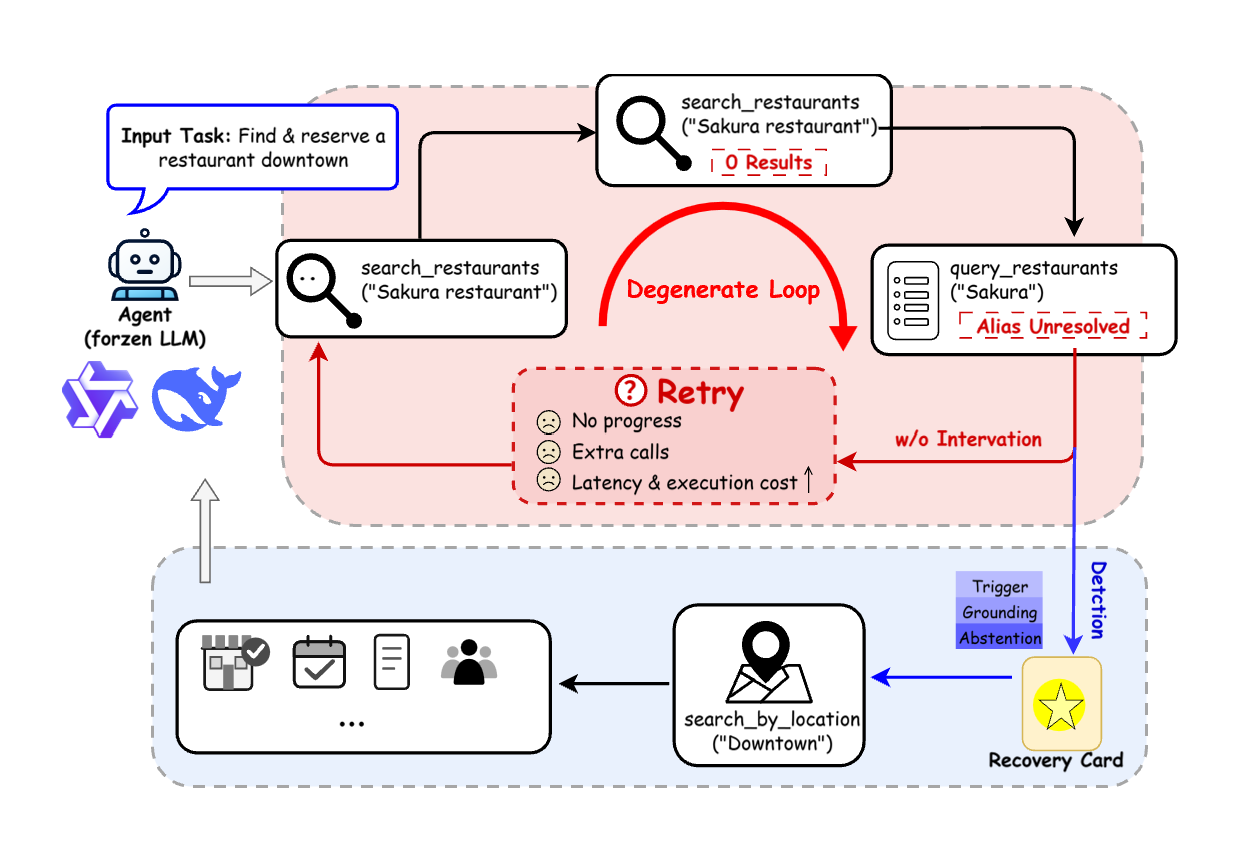
\includegraphics[width=\columnwidth]{figures/fig_persist_ace_escape_overview.png}
    \caption{Illustrative Functional Loop and local escape. After earlier feedback is
    visible, different search and query calls repeat the same unresolved effect
    without progress. PERSIST-ACE admits a grounded location-search Card, makes
    one bounded correction, and returns control to the base LLM.}
    \label{fig:escape-example}
\end{figure}

Existing defenses leave a gap. Exact-repeat blockers miss surface-diverse
failures, early stopping abandons states that may still be recoverable, and
online replanning adds another generation step without guaranteeing a grounded
action. Detection alone is also insufficient: a retry may still be productive,
and some stalled states have no unique safe repair.

We present \textbf{PERSIST-ACE}, which learns bounded recovery programs from
earlier failures. Figure~\ref{fig:framework} shows the full path. Offline, it
compiles recurring effect-level failure patterns into typed Recovery Cards
with explicit triggers, grounding rules, abstention conditions, and budgets.
Online, no-progress recalls a candidate, repeated effect confirms a Functional Loop, and
the controller either admits one grounded Card or preserves the Raw action.
Control then returns to the base LLM without updating its policy or invoking
open-ended replanning.

We evaluate PERSIST-ACE on STATE-Bench, DeepPlanning Shopping, and
$\tau$-Knowledge. The method improves the primary task outcome on all three
benchmarks, and the mechanism study attributes the strongest recovery behavior
to selective, grounded Cards rather than detection or generic prompting alone.

Our contributions are threefold:
\begin{itemize}
    \item \textbf{Functional Loop analysis.} We formalize a Functional Loop as no progress
    plus a feedback-visible repeated functional effect, characterize how it
    varies by model and benchmark, and show why tool-name repetition
    is an inadequate proxy.
    \item \textbf{Programmatic action recovery.} We introduce PERSIST-ACE, an
    offline experience compiler and online selective controller for grounded,
    bounded recovery programs.
    \item \textbf{Evaluation.} We show improved primary task outcomes on three
    tool-use benchmarks and use controlled ablations to separate Card
    validation, grounding, and recovery-program effects.
\end{itemize}

\section{Related Work}



\paragraph{Tool-using LLMs and execution feedback.}
ReAct interleaves language reasoning with environment actions
\citep{yao2023react}, while Toolformer and ToolLLM study how language models
can acquire and invoke external tools \citep{schick2023toolformer,qin2023toollm}.
This line of work primarily addresses action selection and tool-use
capability. PERSIST-ACE starts from an already operational tool-using LLM and
focuses on a later execution problem: a syntactically plausible action can
continue to produce no new evidence, no task-relevant state change, or the
same unresolved functional effect.

\paragraph{Execution recovery and loop handling.}
Early-exit methods reduce repetitive or ineffective behavior by deciding when
to halt, but termination alone does not repair a recoverable task state
\citep{lu2025runaway}. Other approaches generate recovery plans at test time,
as in Reasoning Inception \citep{kim2026rein}, or update the LLM policy so
that it learns from execution errors, as in Fission-GRPO
\citep{zhang2026fission}. PERSIST-ACE takes a narrower and more conservative
route: it does not terminate every loop, invoke an open-ended planner, or
update model parameters at inference time. Instead, it applies at most one
frozen, grounded, deterministic correction when the trigger and safety gates
pass, and preserves the Raw action when grounding is ambiguous or a retry may
still be productive. Unlike early-exit, generative replanning, or policy
optimization, its central object is a selective programmatic escape from a
feedback-visible Functional Loop.

\section{Functional Loops in Tool-Using LLMs}
\label{sec:functional-loops}

We call a feedback-visible sequence a Functional Loop when it makes no task
progress while repeating the same unresolved functional effect. This excludes
both brief inactivity and productive retries.

\textbf{Definition.} Consider a tool-use trajectory
$\tau=(s_0,a_0,o_0,\ldots,s_T)$, where $s_t$ is the online-visible interaction
state, $a_t$ is the proposed tool action, and $o_t$ is the resulting observation.
We summarize the visible task state as
\begin{equation}
q_t=(E_t,S_t,U_t),
\end{equation}
where $E_t$ is non-redundant evidence, $S_t$ is the task-relevant environment
state, and $U_t$ contains unresolved user requirements. The action effect is
\begin{equation}
e_t=(\Delta E_t,\Delta S_t,\Delta U_t,f_t),
\end{equation}
where $f_t$ records an execution or semantic failure. The mapping
$\kappa(e_t)$ canonicalizes changes to evidence, task state, unresolved
requirements, and the blocking failure.

Let $p_t=1$ when $a_t$ adds non-redundant evidence, changes state toward an
unresolved requirement, resolves a requirement, or changes a failure signature
in a way that enables a new action. For the action window
$W_{t,w}=\{t,\ldots,t+w-1\}$, define
\begin{equation}
N(t,w)=\mathbb{I}\!\left[U_t\neq\varnothing\ \land\
\sum_{j\in W_{t,w}}p_j=0\right]
\end{equation}
and
\begin{equation}
R_e(t,w)=\mathbb{I}\!\left[
\substack{\exists i<j,\ i,j\in W_{t,w}:\\
\kappa(e_i)=\kappa(e_j)\ \land\ o_i\prec a_j}
\right],
\end{equation}
where $o_i\prec a_j$ means that the earlier tool result was visible before the
later action was proposed. The strict definition is
\begin{equation}
\mathcal{L}(t,w)=N(t,w)\land R_e(t,w).
\label{eq:functional-loop}
\end{equation}
Here $N=1$ recalls a candidate, whereas $\mathcal{L}=1$ also requires a repeated
effect after feedback is visible. A loop is \emph{recoverable} only when a
Card passes grounding, abstention, and safety checks, and \emph{triggered} only
when that Card is executed. A trajectory is \emph{Functional Loop-exposed} if
it contains at least one episode. Tool strings are not part of the definition:
different tools may repeat an effect, while another call to the same tool may
produce new evidence.

\textbf{Functional Loop variation by model and benchmark.}
Figures~\ref{fig:statebench-model-fl} and~\ref{fig:cross-benchmark-fl} separate
two sources of variation. On the same failed STATE-Bench tasks, Qwen3-14B
loops more often than DeepSeek-v4-Flash, MiMo-v2.5-Pro, or DeepSeek-v4-Pro.
With DeepSeek-v4-Flash held fixed, prevalence is highest on DeepPlanning
Shopping, lower on $\tau$-Knowledge, and lowest on STATE-Bench. Functional
Loops therefore depend on both the model's tool policy and the environment.

\begin{figure}[t]
  \centering
  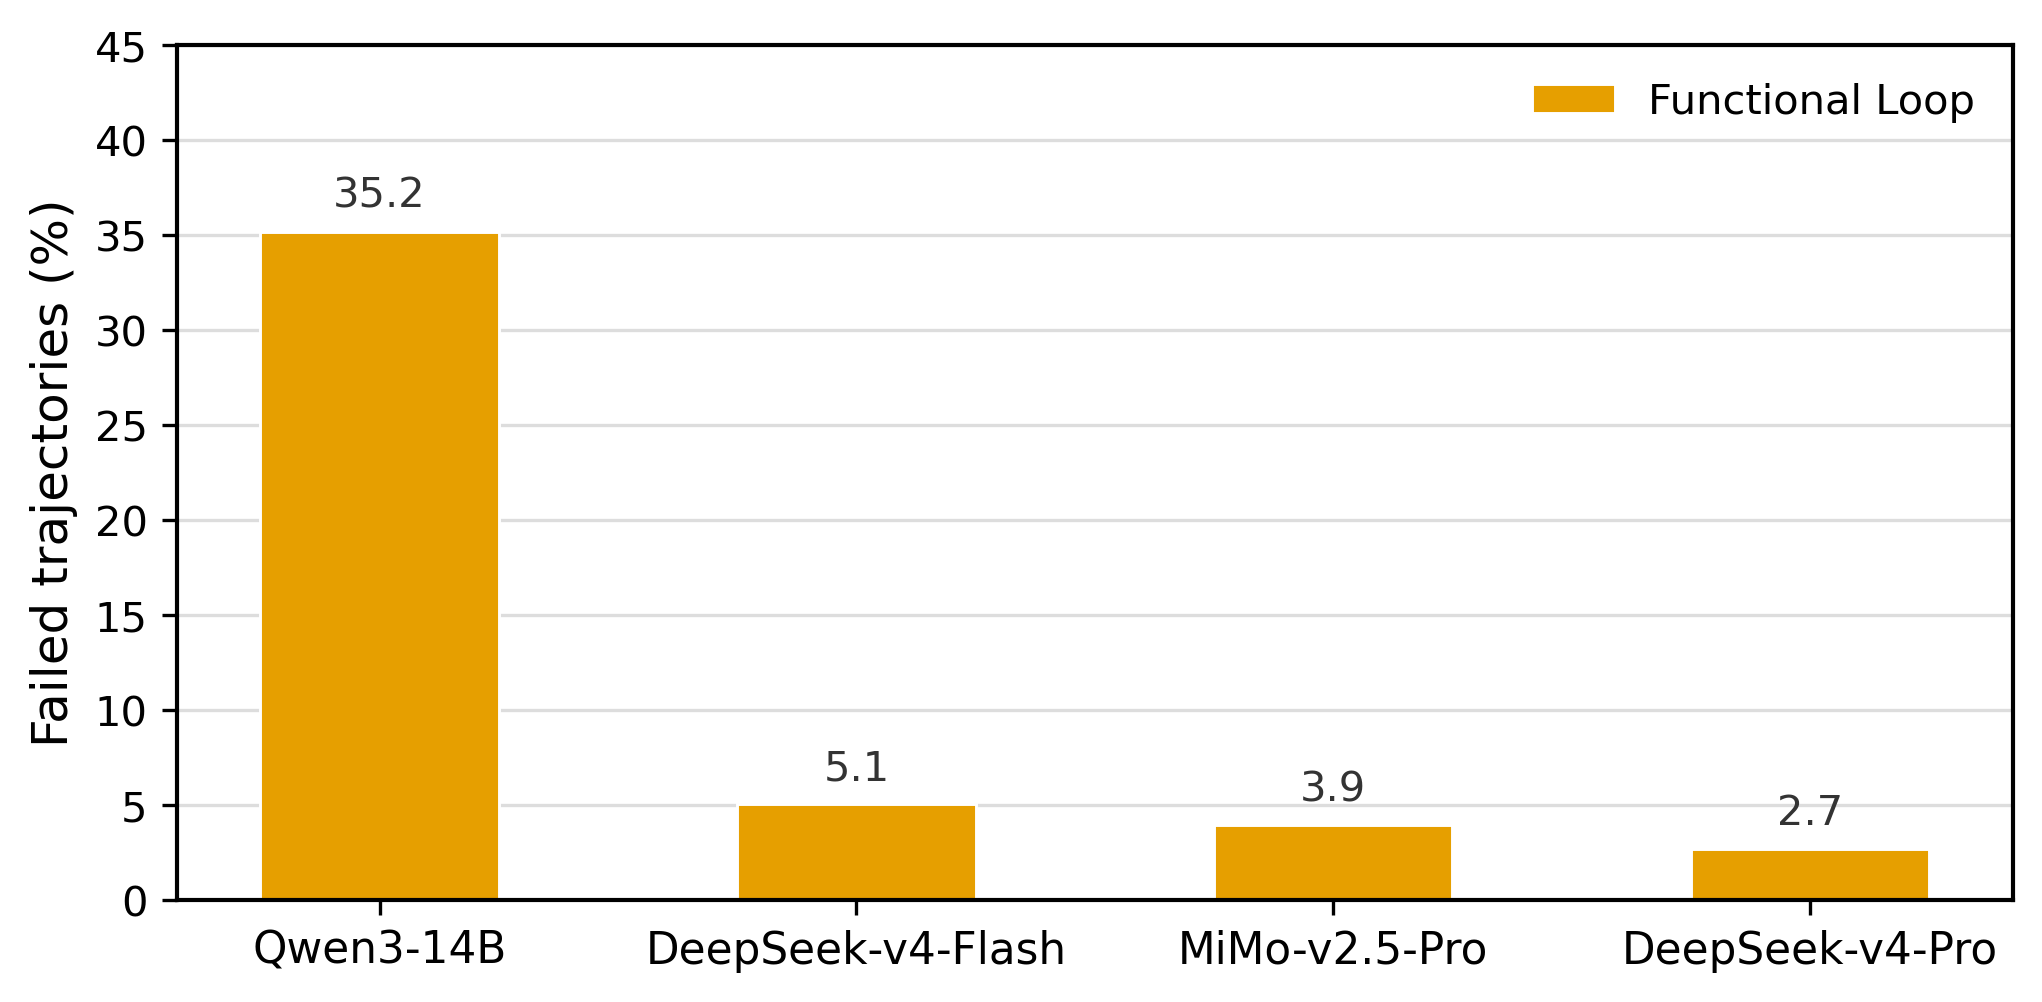
\includegraphics[width=\columnwidth]{figures/fig_statebench_fl_or_invalid_models.png}
  \caption{Functional Loop prevalence among failed STATE-Bench trajectories
  for four tool-using LLMs.}
  \label{fig:statebench-model-fl}
\end{figure}

\begin{figure}[t]
  \centering
  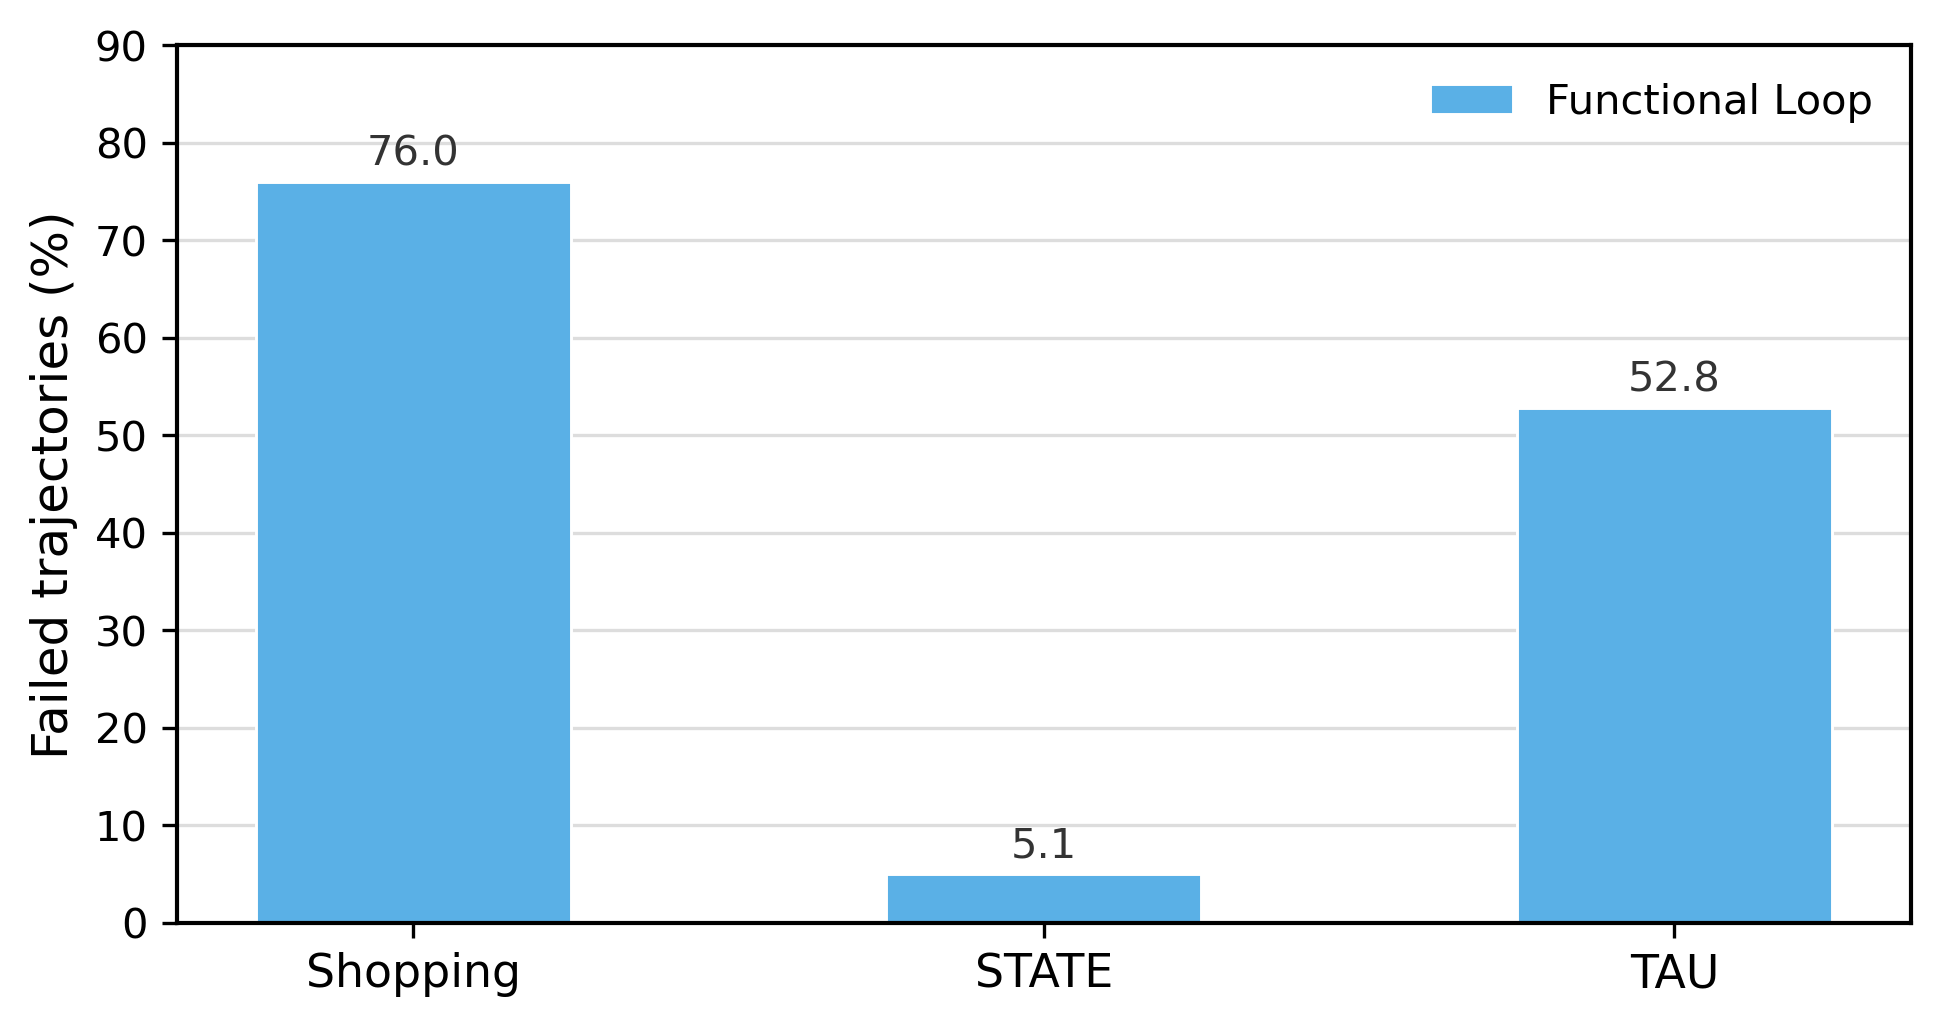
\includegraphics[width=\columnwidth]{figures/fig_cross_benchmark_fl_fixed_agent.png}
  \caption{Functional Loop prevalence among failed DeepSeek-v4-Flash
  trajectories on three benchmarks.}
  \label{fig:cross-benchmark-fl}
\end{figure}

\textbf{Functional Loops, outcomes, and cost.}
On STATE-Bench, Functional Loop-exposed trajectories have lower scores and use
more tool calls for every evaluated model
(Figure~\ref{fig:statebench-fl-consequence}). This is an observational
association: difficult tasks may both invite longer interaction and fail more
often. Even so, the pattern identifies a costly execution state worth
recovering from.

\begin{figure}[t]
  \centering
  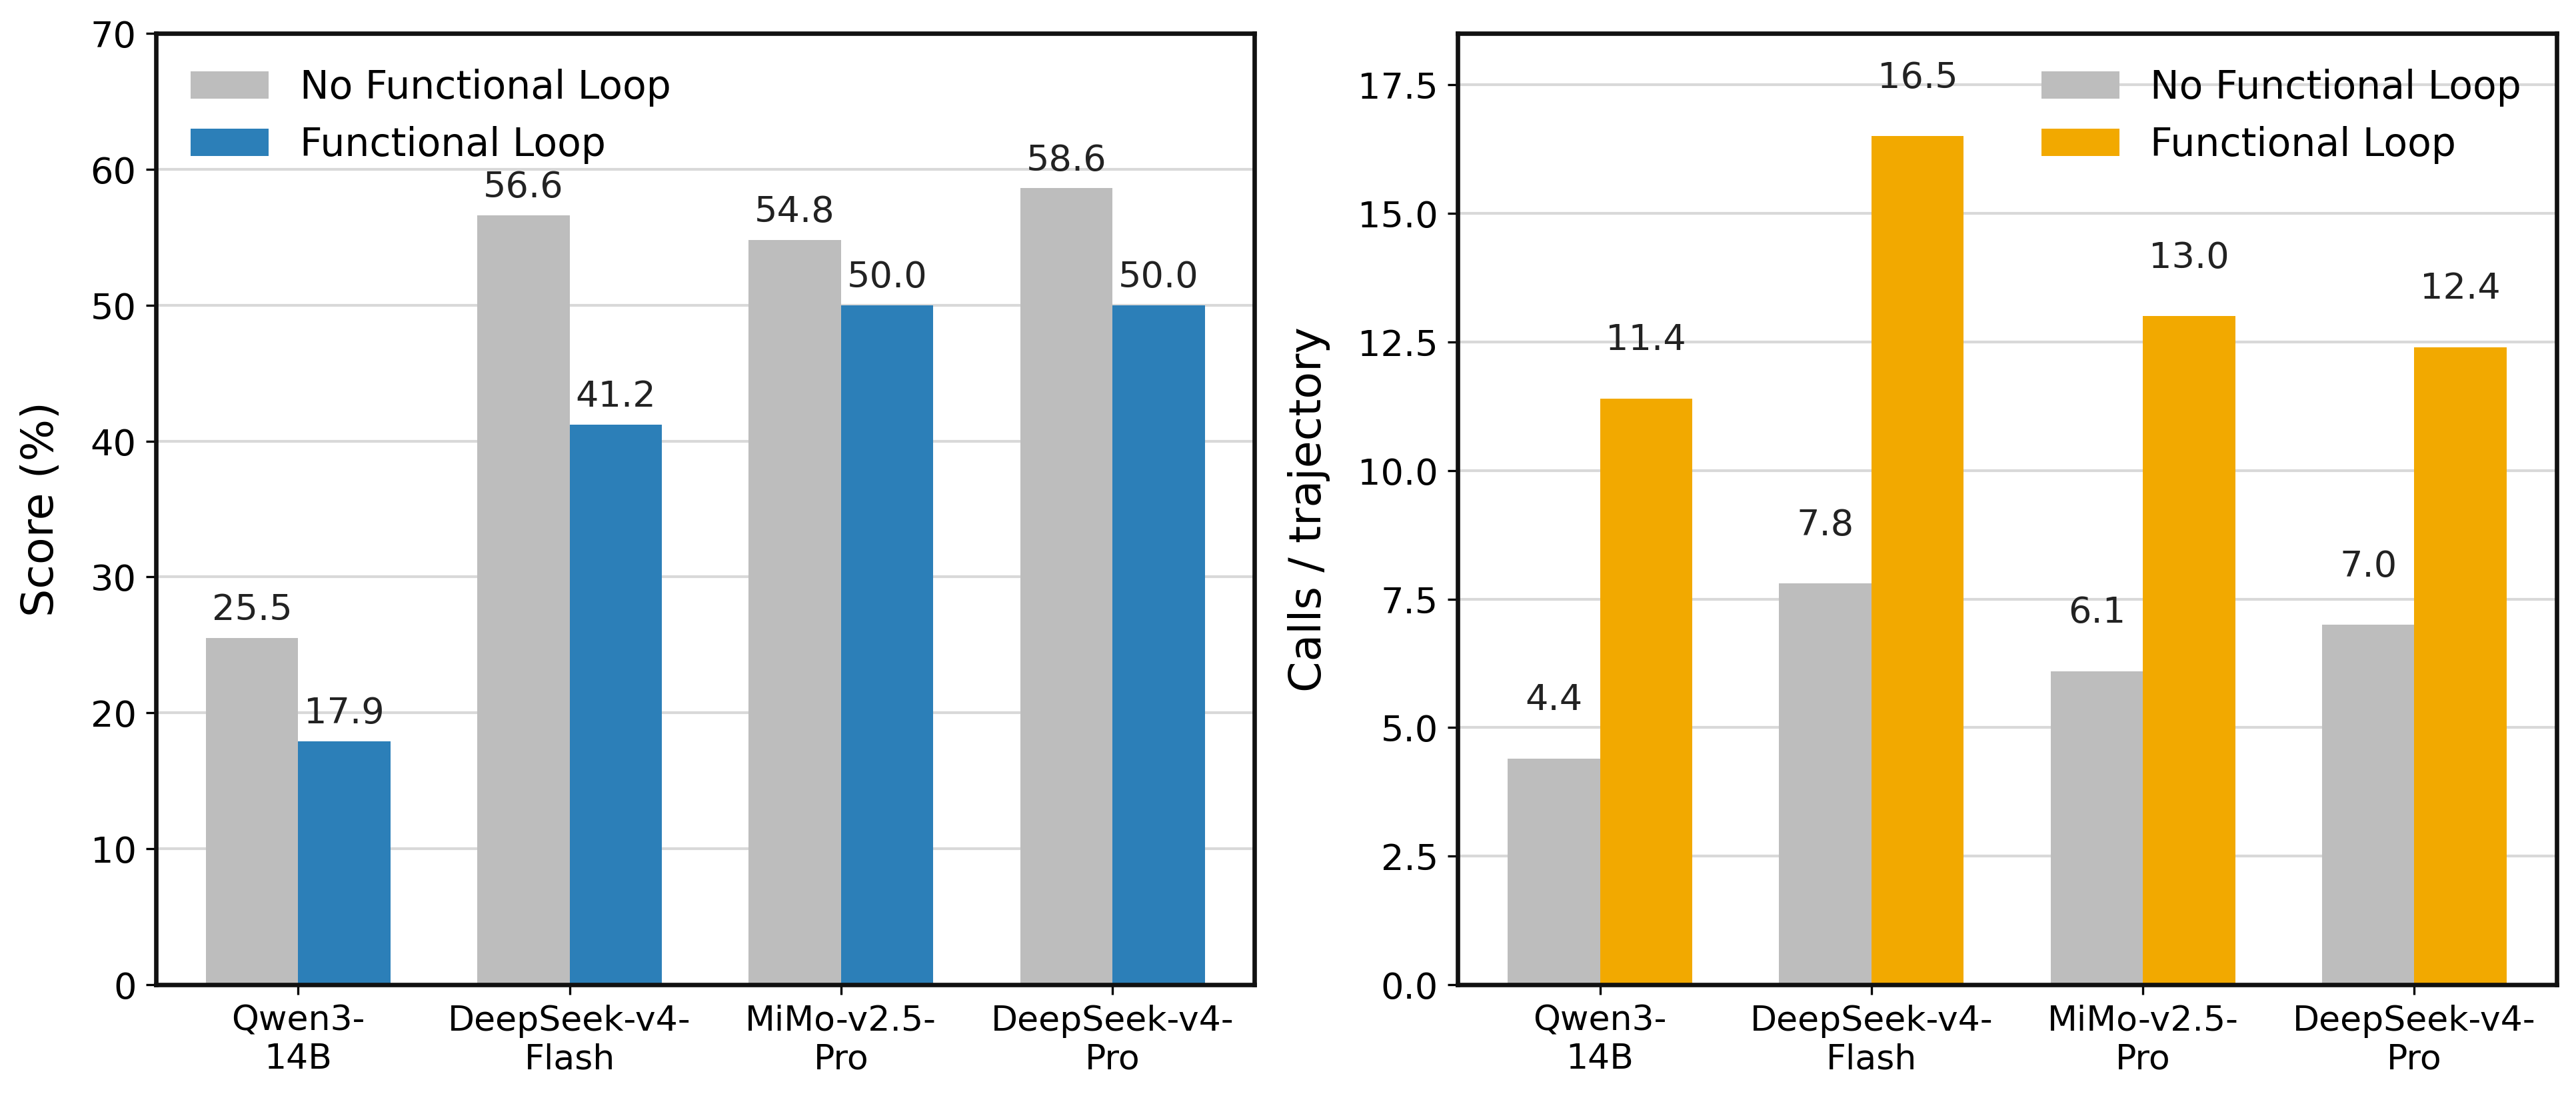
\includegraphics[width=\columnwidth]{figures/fig_fl_statebench_consequences.png}
  \caption{STATE-Bench outcomes and tool calls grouped by Functional Loop
  exposure. }
  \label{fig:statebench-fl-consequence}
\end{figure}

Consecutive reuse of the same tool gives a weaker signal
(Figure~\ref{fig:same-tool-repeat}): score differences are small and change
direction across models. Functional effects, rather than action strings,
provide the useful boundary.

\begin{figure}[t]
  \centering
  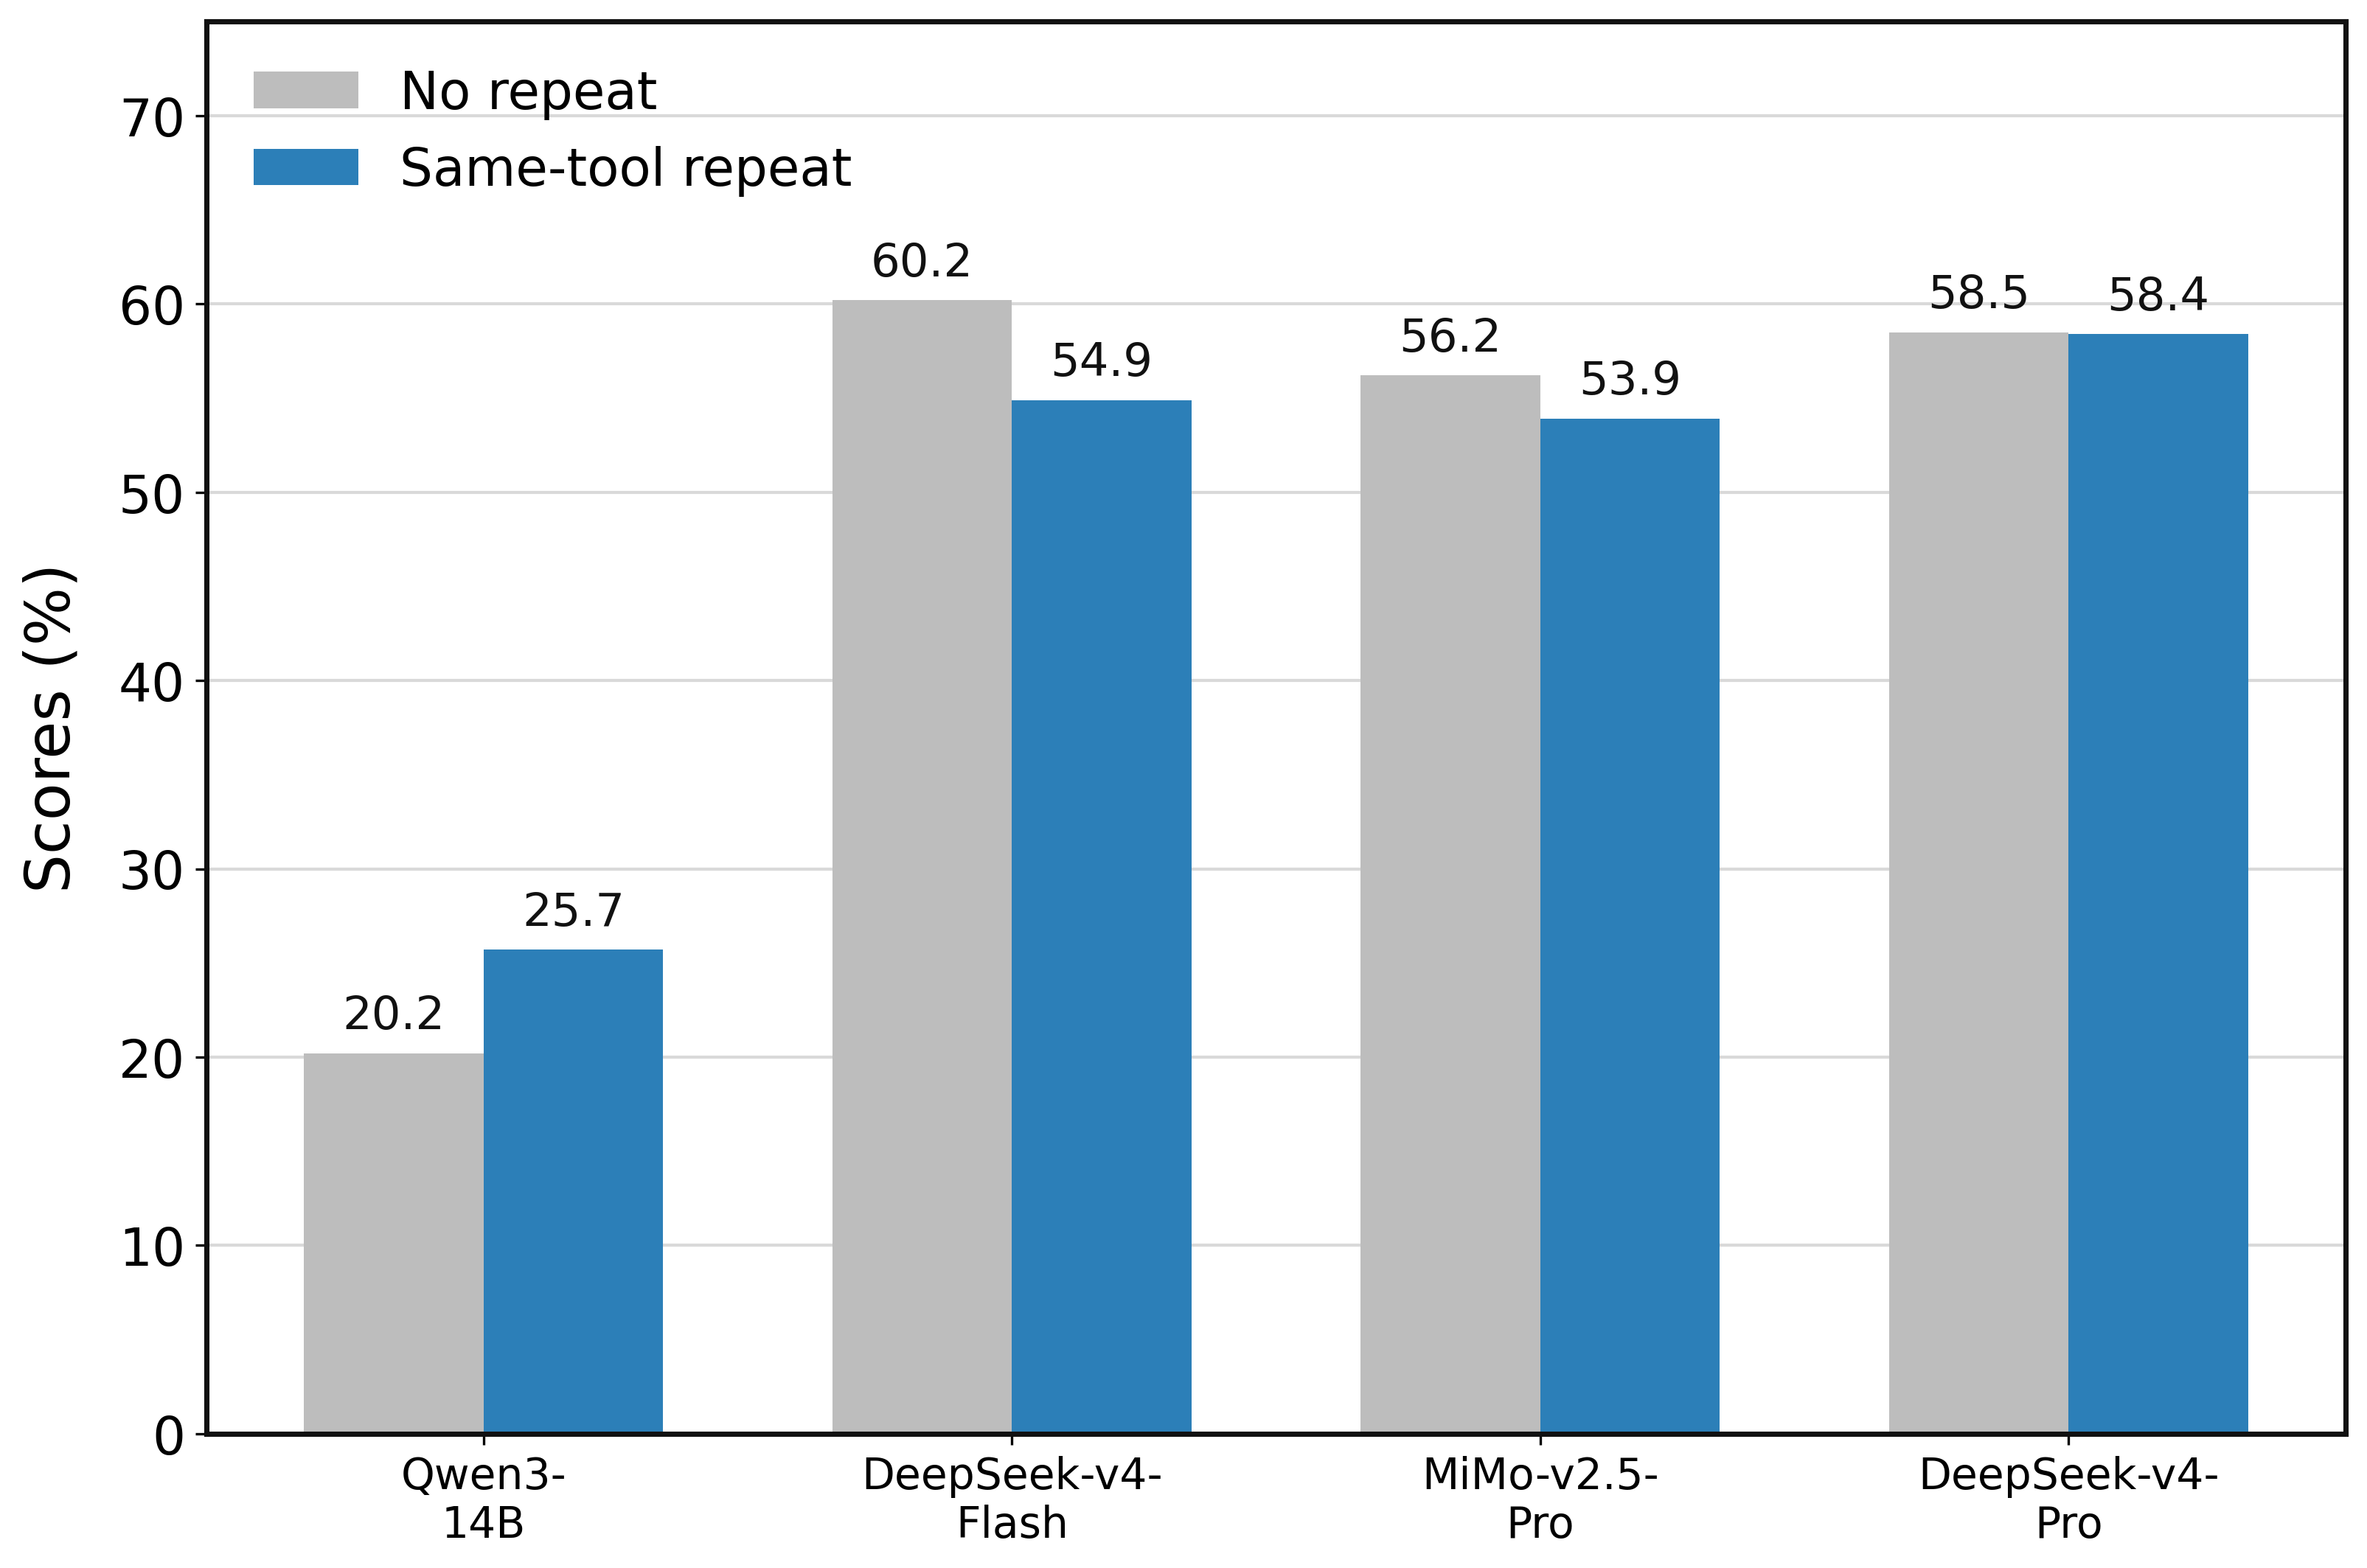
\includegraphics[width=\columnwidth]{figures/fig_statebench_same_tool_repeat.png}
  \caption{Raw STATE-Bench score grouped by consecutive calls with the same
  tool name. String-level repetition is a weak proxy for unresolved effect.}
  \label{fig:same-tool-repeat}
\end{figure}

\textbf{Case study: a cross-tool Functional Loop.}
Table~\ref{tab:cross-tool-fl-case} traces a Raw STATE-Bench Shopping
trajectory in which DeepSeek-v4-Flash searches for wireless headphones under
a hard \$100 budget. Two valid searches find nothing; the LLM then retrieves a
\$110 item and checks its details, the account, and promotions. The tools
change, but none resolves the budget constraint.

\begin{table}[t]
\centering
\scriptsize
\setlength{\tabcolsep}{2pt}
\begin{tabular}{@{}p{0.08\columnwidth}p{0.29\columnwidth}p{0.28\columnwidth}p{0.27\columnwidth}@{}}
\toprule
Step & Tool action & Feedback & Functional effect \\
\midrule
1--2 & \texttt{search\_products} ($\leq\$100$) & No matching headphones & No feasible item \\
3 & \texttt{search\_products} ($\leq\$1000$) & Finds a \$110 candidate & Budget violated \\
4 & \texttt{get\_product}\newline\texttt{\_details} & Confirms the \$110 price & Violation persists \\
5--6 & Account and promotion queries & No benefit or discount & Constraint unresolved \\
\bottomrule
\end{tabular}
\caption{A cross-tool Functional Loop from STATE-Bench Shopping. Different
calls repeat the same unresolved budget effect after feedback is visible.}
\label{tab:cross-tool-fl-case}
\end{table}

The first searches are productive because they may reveal a feasible item. The
loop begins only after the over-budget candidate is known and subsequent checks
add no repair evidence. It is a recovery signal, not an automatic stop command.

\textbf{From Functional Loop signals to recovery.}
No progress recalls a candidate; a feedback-visible repeated effect establishes
the loop; admission then asks whether a unique, grounded repair is available.
PERSIST-ACE executes one bounded Card only when these checks pass and then
returns control to the LLM. Figure~\ref{fig:escape-example} illustrates the
escape, while Figure~\ref{fig:framework} implements it as
Observe--Detect--Admit--Recover.

\section{PERSIST-ACE}
\label{sec:method}

PERSIST-ACE is a local recovery layer for tool-using LLMs. As shown in
Figure~\ref{fig:framework}, its offline path compiles training failures into a
frozen Registry, while its online path detects a Functional Loop, admits one
grounded Recovery Card, and returns the resulting observation to the LLM.
Compilation is run independently for each benchmark; trajectories and Cards are
not pooled across benchmarks. PERSIST-ACE neither updates the base model nor
replaces its global planner.

\begin{figure*}[t]
\centering
\IfFileExists{figures/fig_persist_ace_pipeline.png}{%
  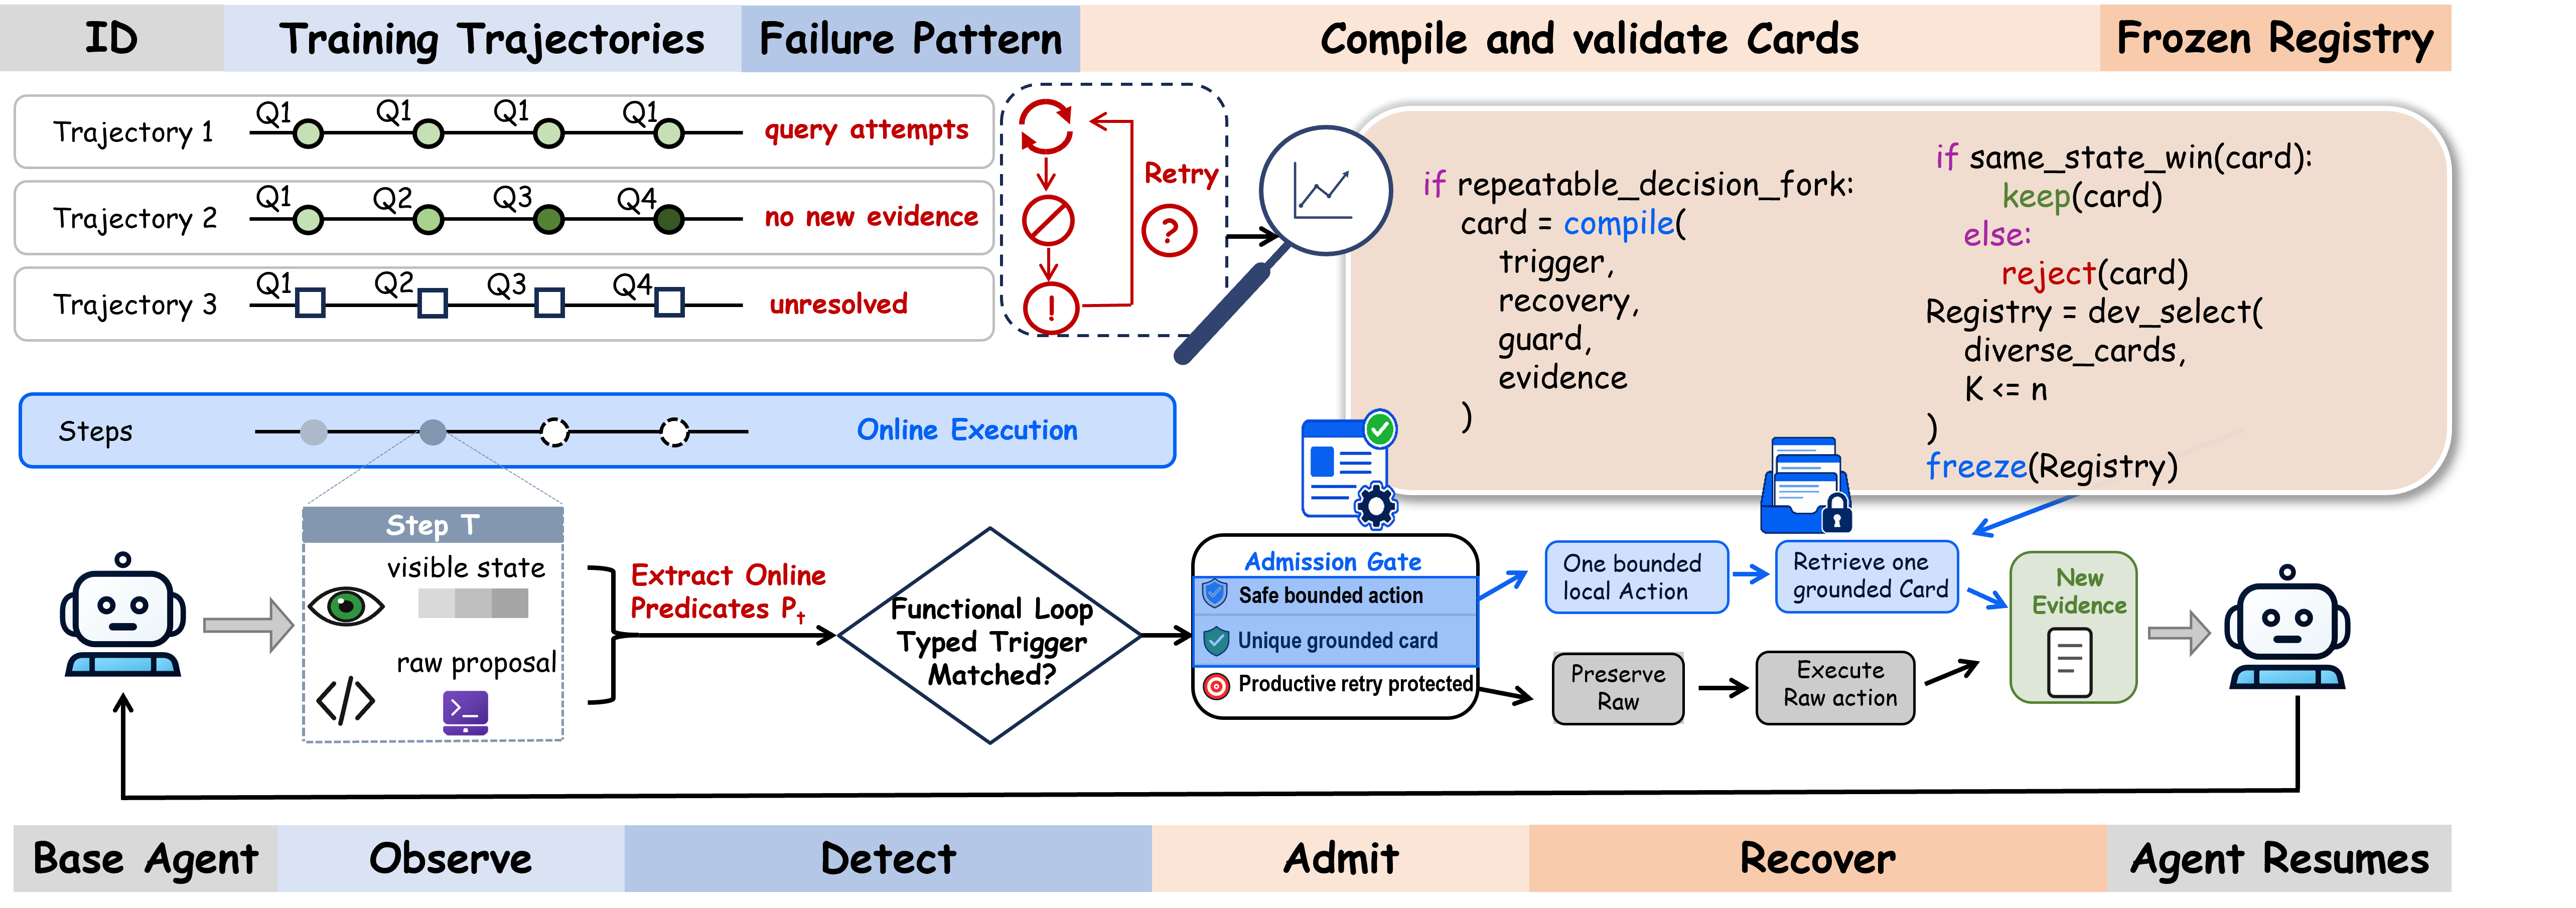
\includegraphics[width=0.97\textwidth]{figures/fig_persist_ace_pipeline.png}%
}{%
  \fbox{\parbox{0.95\textwidth}{\centering\small
  \textbf{Offline:} Raw training trajectories $\rightarrow$ suspicious
  pre-action states $\rightarrow$ effect/state clusters $\rightarrow$
  schema-grounded candidates $\rightarrow$ execution validation $\rightarrow$
  frozen benchmark-specific Registry
  \quad $\mid$ \quad
  \textbf{Online:} Raw proposal $+$ visible state $\rightarrow$
  trigger and guard checks $\rightarrow$ grounded recovery or Raw action}}
}
\caption{PERSIST-ACE compiles benchmark-specific training failures into a
frozen Registry. Online, it observes the state and Raw proposal, detects a
Functional Loop, admits a grounded and safe Card, executes one bounded
recovery, and returns control to the LLM.}
\label{fig:framework}
\end{figure*}

\subsection*{Offline Experience Compilation}

\textbf{Mine failure patterns.} The upper path of
Figure~\ref{fig:framework} starts from one benchmark's training trajectories.
At each pre-action prefix, $N$ recalls a no-progress state and $\kappa(e)$ tests
whether feedback-visible calls repeat the same unresolved effect. Only states
satisfying Eq.~\ref{eq:functional-loop} are Functional Loops. Other local
failures may inform recovery construction without being relabeled as loops. We
represent a candidate as
\begin{equation}
x_i=\left(s_i,a_i,e_i,\Delta E_i,\Delta S_i,u_i,\hat a_i,g_i,r_i\right),
\label{eq:candidate}
\end{equation}
where $\hat a_i$ is an executable replacement, $g_i$ its visible grounding
source, and $r_i$ a risk tag. Replacements may repair an argument, tool choice,
or blocked prerequisite, but cannot invent entities or relax user constraints.
Candidates are grouped by unresolved effect, requirement, action transition,
replacement, and grounding source.

\textbf{Compile and validate Cards.} Each supported group is compiled into a
Typed Recovery Card
\begin{equation}
c=(z_c,\phi_c,\psi_c,\rho_c,g_c,b_c,r_c),
\label{eq:card}
\end{equation}
where $z_c$ identifies the failure family, $\phi_c$ the trigger, $\psi_c$ the
abstention guards, $\rho_c$ the executable program, $g_c$ its grounding rule,
$b_c$ its budget, and $r_c$ its role and risk. Thus, a Card is a typed local
program rather than free-form advice. When snapshots are available, Raw and
Card actions are compared from the same state; otherwise we use paired or
repeated execution without claiming same-state evidence. Validation uses task
outcome and execution validity, while loop and cost measures remain
diagnostics.

\textbf{Freeze the Registry.} We reject candidates that require future or test
information, ambiguous entities, or constraint violations. Training-time
induction is protocol-constrained and LLM-assisted: a coding LLM may normalize
training failures and instantiate the fixed Card schema, but retention follows
the prescribed grounding, safety, validation, and development gates.
Researchers set this protocol without accessing test tasks or outcomes. Card
definitions, priorities, budgets, effect canonicalization, and controller
settings are frozen before test execution.

\subsection*{Online Selective Recovery}

\textbf{Observe and detect.} In the lower path of
Figure~\ref{fig:framework}, the LLM receives tool feedback and proposes Raw
action $a_t$. Observe exposes the visible history and state $s_t$: effects,
evidence changes, unresolved requirements, constraints, and the proposal.
Detect applies Eq.~\ref{eq:functional-loop}; $N=1$ recalls no progress and
$R_e=1$ confirms a repeated feedback-visible effect. It uses no future outcome.
A repeated tool name is insufficient, and detection alone does not authorize
intervention.

\textbf{Admit.} The controller next retrieves Cards whose trigger matches the
current Functional Loop family. Let the eligible set at step $t$ be
\begin{equation}
\begin{aligned}
\mathcal{C}_t=\{c\in\mathcal{R}:{}&\phi_c(s_t,a_t)=1
\land\psi_c(s_t,a_t)=0,\\
&b_c>0\land\operatorname{Unique}(g_c(s_t))=1,\\
&\operatorname{Safe}(\rho_c(s_t,a_t))=1\}.
\end{aligned}
\label{eq:eligible}
\end{equation}
where $\phi_c$ matches the state and effect, $\psi_c$ protects productive
retries, and $b_c$ is the remaining budget. Admission also requires unique
grounding and a schema-valid, constraint-preserving action. A frozen priority
order favors smaller changes, stronger grounding, validation support, and
lower risk. Recent progress, a productive retry, ambiguity, conflict, budget
exhaustion, or a failed safety check preserves the Raw proposal.

\textbf{Recover and resume.} For the highest-priority admitted Card
$c^\star$, the executed policy is
\begin{equation}
\pi_{\mathrm{ACE}}(s_t,a_t)=
\begin{cases}
\rho_{c^\star}(s_t,a_t), & \mathcal{C}_t\neq\varnothing,\\
 a_t, & \mathcal{C}_t=\varnothing,
\end{cases}
\label{eq:controller}
\end{equation}
The environment executes the bounded Card program or the Raw action and returns
a new observation. Control then returns to the LLM. Cards cannot invoke one
another without an intervening LLM proposal, and recovery does not guarantee
task success. Functional Loop detection locates an opportunity; admission
decides whether and how to act.

\FloatBarrier
\section{Experiments}
\label{sec:experiments}

\begin{table*}[!t]
\centering
\small
\setlength{\tabcolsep}{3pt}
\renewcommand{\arraystretch}{0.95}
\begin{tabular*}{\textwidth}{@{\extracolsep{\fill}}llrrrrrr@{}}
\toprule
Setting & Model & Pass@1 (\%) & $\Delta$ & Pass$^5$ (\%) & $\Delta$ & UX & $\Delta$ \\
\midrule
Raw & Ministral-3-14B & 30.5 & -- & 8.7 & -- & 2.95 & -- \\
Raw & Qwen3-14B & 24.0 & -- & 7.3 & -- & 2.90 & -- \\
Raw & GPT-5.5 & 56.67 & -- & 34.00 & -- & 3.760 & -- \\
Raw & Claude-Sonnet-5 & 62.00 & -- & 36.67 & -- & 4.065 & -- \\
Raw & Claude-Opus-4-8 & 57.47 & -- & 30.00 & -- & 4.022 & -- \\
Raw & DeepSeek-v4-Flash & 56.9 & -- & 30.0 & -- & 3.72 & -- \\
Raw & DeepSeek-v4-Pro & 59.1 & -- & 34 & -- & 3.93 & -- \\
Raw & MiMo-v2.5-pro & 54.5 & -- & 27.3 & -- & 3.96 & -- \\
Raw & GPT-5.6-Sol & 62.13 & -- & 39.33 & -- & 3.927 & -- \\
PERSIST-ACE & Ministral-3-14B & 30.9 & +0.4 & 11.3 & +2.6 & 2.96 & +0.01 \\
PERSIST-ACE & Qwen3-14B & 26.8 & +2.8 & 10.0 & +2.7 & 2.90 & 0 \\
PERSIST-ACE & GPT-5.5 & 60.80 & +4.13 & 35.33 & +1.33 & 3.788 & +0.028 \\
PERSIST-ACE & Claude-Sonnet-5 & 62.80 & +0.80 & 36.00 & -0.67 & 4.047 & -0.018 \\
PERSIST-ACE & Claude-Opus-4-8 & 59.33 & +1.86 & 30.67 & +0.67 & 4.052 & +0.030 \\
PERSIST-ACE & DeepSeek-v4-Flash & 59.5 & +2.5 & 34.0 & +4.0 & 3.75 & +0.03 \\
PERSIST-ACE & DeepSeek-v4-Pro & 59.5 & +0.4 & 34.0 & 0 & 3.94 & +0.01 \\
PERSIST-ACE & MiMo-v2.5-pro & 56.3 & +1.7 & 27.3 & 0 & 3.96 & 0 \\
PERSIST-ACE & GPT-5.6-Sol & 62.67 & +0.54 & 38.67 & -0.66 & 3.959 & +0.032 \\
\bottomrule
\end{tabular*}
\renewcommand{\arraystretch}{1.0}
\caption{Overall STATE-Bench test results. Each setting contains 150 tasks and
five trials, with a fixed 750-trajectory Pass@1 denominator. $\Delta$ denotes
PERSIST-ACE minus Raw; UX averages valid judged trajectories.}
\label{tab:state-main}
\end{table*}

\begin{table*}[!t]
\centering
\small
\setlength{\tabcolsep}{3pt}
\renewcommand{\arraystretch}{0.95}
\begin{tabular*}{\textwidth}{@{\extracolsep{\fill}}llrrrr@{}}
\toprule
Setting & Model & Match Score (\%) & $\Delta$ & Case Acc. (\%) & $\Delta$ \\
\midrule
Raw & Qwen3-14B & 40.051 & -- & 6.250 & -- \\
Raw & DeepSeek-v4-Flash & 83.720 & -- & 52.917 & -- \\
Raw & DeepSeek-v4-Pro & 82.329 & -- & 51.667 & -- \\
PERSIST-ACE & Qwen3-14B & 42.063 & +2.012 & 6.458 & +0.208 \\
PERSIST-ACE & DeepSeek-v4-Flash & 84.811 & +1.090 & 54.375 & +1.458 \\
PERSIST-ACE & DeepSeek-v4-Pro & 83.781 & +1.452 & 55.625 & +3.958 \\
\bottomrule
\end{tabular*}
\renewcommand{\arraystretch}{1.0}
\caption{Overall DeepPlanning Shopping test results. Each setting contains
120 tasks and four trials (480 task-runs). $\Delta$ denotes PERSIST-ACE minus
Raw.}
\label{tab:deepplanning-main}
\end{table*}

We compare Raw tool-using LLMs with the same models equipped with PERSIST-ACE. Official
task measures are primary; Functional Loop behavior and tool use are reported as execution
diagnostics.

\subsection*{Benchmarks}

\textbf{STATE-Bench.} STATE-Bench v0.8.1 contains 50 held-out tasks in each of
Travel, Customer Support, and Shopping Assistant. We report Pass@1,
pass$^5$, and UX. Following the official protocol, Pass@1 is the average
task-completion rate over five runs per task, whereas pass$^5$ is the percentage
of tasks completed successfully in all five runs and measures run-to-run
reliability.

\textbf{DeepPlanning.} We use the 120-task Shopping Planning split of
DeepPlanning~\citep{zhang2026deepplanning}, reporting Match Score and Case
Accuracy. Travel Planning is outside this comparison.

\textbf{$\tau$-Knowledge.} This 97-task benchmark evaluates knowledge-intensive
tool use~\citep{shi2026tauknowledge}. We report Reward mean, pass$^1$--pass$^4$,
Action Recall, and Document Recall.

\subsection*{Experimental Setup}

\paragraph{Data separation and freezing protocol.}
We separate Card construction from final evaluation before any test runs. For
STATE-Bench, we keep the official 50-task test split in each domain and split
the original 100 training tasks into 70/30 train/development tasks; for
DeepPlanning Shopping, we use three 60/20/40 train/development/test folds; and
for $\tau$-Knowledge, we rotate three 32/33/32 partitions through the same
roles. Training data mine and instantiate Cards, development data select the
Registry, and all Card definitions and controller settings are frozen before
held-out testing. For folded benchmarks, we report aggregated out-of-fold test
results, with exact manifests and Card provenance in the supplement.

\textbf{STATE-Bench.} We evaluate nine LLMs on all 150 test tasks, with five
runs per task. For each LLM, Raw uses the base model and PERSIST-ACE adds the
same frozen nine-Card Registry. Tasks, tools, simulator, evaluator, and trial
identities are otherwise unchanged.

\textbf{DeepPlanning Shopping.} We evaluate Qwen3-14B,
DeepSeek-v4-Flash, and DeepSeek-v4-Pro on all 120 Shopping tasks, with four
runs per task. For each LLM, Raw uses the base model and PERSIST-ACE adds the
same frozen Shopping Registry. Tasks, tools, and trial identities are otherwise
unchanged.

\textbf{$\tau$-Knowledge.} We evaluate five matched model-version pairs on all
97 tasks, with four runs per task. For each pair, Raw uses the base model and
PERSIST-ACE adds the same frozen knowledge-tool Registry. Tasks, tools, and
trial identities are otherwise unchanged; metrics absent from a stored run are
marked N/R.

Across benchmarks, invalid executions are kept separate from Functional Loop counts and
missing telemetry is never reconstructed from aggregate outcomes.

\begin{table*}[!t]
\centering
\scriptsize
\setlength{\tabcolsep}{1.5pt}
\renewcommand{\arraystretch}{0.95}
\begin{tabular*}{\textwidth}{@{\extracolsep{\fill}}ll*{14}{r}@{}}
\toprule
Setting & Model & Reward (\%) & $\Delta$ & Pass$^1$ (\%) & $\Delta$ & Pass$^2$ (\%) & $\Delta$ & Pass$^3$ (\%) & $\Delta$ & Pass$^4$ (\%) & $\Delta$ & Action Recall (\%) & $\Delta$ & Doc Recall (\%) & $\Delta$ \\
\midrule


Raw & Claude-Sonnet-5  & 18.44 & -- & 16.24 & -- & 11.00 & -- & 7.99 & -- & 5.15 & -- & 66.02 & -- & 70.29 & -- \\
Raw & Claude-Opus-4-8  & 18.29 & -- & 17.27 & -- & 10.65 & -- & 7.22 & -- & 5.15 & -- & 68.12 & -- & 62.15 & -- \\
Raw & GPT-5.5 & 20.11 & -- & 20.05 & -- & 14.58 & -- & 10.22 & -- & 8.14 & -- & 51.46 & -- & 65.29 & -- \\
Raw & DeepSeek-v4-Flash & 20.10 & -- & 20.10 & -- & 12.37 & -- & 9.79 & -- & 8.25 & -- & 72.97 & -- & 70.35 & -- \\
Raw & GPT-5.6-Sol  & 20.11 & -- & 20.79 & -- & 13.89 & -- & 10.90 & -- & 8.75 & -- & 51.27 & -- & 72.01 & -- \\


PERSIST-ACE & Claude-Sonnet-5  & 18.69 & +0.25 & 17.01 & +0.77 & 11.28 & +0.28 & 8.19 & +0.20 & 6.12 & +0.97 & 66.70 & +0.68 & 70.55 & +0.26 \\
PERSIST-ACE & Claude-Opus-4-8 & 20.11 & +1.82 & 20.10 & +2.83 & 14.34 & +3.69 & 11.66 & +4.44 & 10.08 & +4.93 & 51.22 & -16.90 & 68.65 & +6.50 \\
PERSIST-ACE & GPT-5.5 & 21.94 & +1.83 & 22.16 & +2.11 & 15.02 & +0.44 & 11.74 & +1.52 & 9.92 & +1.78 & 52.24 & +0.78 & 68.03 & +2.74 \\
PERSIST-ACE & DeepSeek-v4-Flash & 20.88 & +0.77 & 20.88 & +0.77 & 13.06 & +0.69 & 10.05 & +0.26 & 8.25 & +0.00 & 75.11 & +2.13 & 71.35 & +1.00 \\
PERSIST-ACE & GPT-5.6-Sol  & 25.46 & +5.36 & 25.86 & +5.07 & 18.40 & +4.51 & 13.03 & +2.13 & 10.00 & +1.25 & 52.35 & +1.08 & 72.89 & +0.88 \\
\bottomrule
\end{tabular*}
\renewcommand{\arraystretch}{1.0}
\caption{Overall $\tau$-Knowledge test results. Each setting contains 97 tasks
and four trials (388 task-runs). $\Delta$ denotes PERSIST-ACE minus Raw.}
\label{tab:tau-main}
\end{table*}

\subsection*{Main Results}

\textbf{STATE-Bench.} Table~\ref{tab:state-main} covers nine models spanning
open and proprietary model families and a wide range of Raw performance.
Every paired comparison improves Pass@1. The repeated-trial measure improves
or holds for seven models, and UX is non-decreasing for eight. The strongest
gains are not confined to either the weakest or strongest baseline, which
argues against a single-model or simple ceiling explanation. The smaller
movements in repeated-trial performance and UX also show that the main benefit
is better task completion, not a uniform shift in every judged outcome.

\textbf{DeepPlanning Shopping.} Table~\ref{tab:deepplanning-main} provides a
different test: long-horizon product search and planning rather than
interactive service tasks. All three models improve both matching quality and
case-level completion, with no execution errors in either arm. The size of the
gain varies by model, but its direction is consistent. This matters because
the Shopping Registry is benchmark-specific while the recovery mechanism is
unchanged, suggesting that the same compilation-and-control design can carry
different local experience.

\textbf{$\tau$-Knowledge.} Table~\ref{tab:tau-main} extends the comparison to
knowledge-intensive tool use. Reward improves for every matched model-version
pair, and all reported pass-rate differences are non-negative. Document recall
also rises throughout. Auxiliary behavior is not uniformly better---most
Action Recall values increase, but one model shows a marked decline---so the
evidence supports better end-task performance rather than dominance on every
intermediate diagnostic.

Taken together, the three tables show the same top-level pattern across
different tools, task horizons, and model families: selective recovery raises
the native task outcome without relying on a single benchmark or model. The
remaining variation is concentrated in secondary measures, which is expected
from a sparse local intervention that changes only eligible portions of a
trajectory.

\section{Ablations and Recovery Analysis}
\label{sec:analysis}

We test whether the gains require compiled Cards, Registry validation, grounded
arguments, and selective admission.

\subsection*{Ablation Studies}

Tables~\ref{tab:compiled-selection} and
\ref{tab:controller-gate-ablation} evaluate full test trajectories;
Table~\ref{tab:card-structure-ablation} uses same-state forks.

\textbf{Prompts and Registry validation.}
Table~\ref{tab:compiled-selection} replaces Cards with generic reconsideration
prompts at Functional Loop or exact-repeat triggers. Neither improves on Raw.
The unvalidated Registry does improve task outcomes, but intervenes more often
and incurs more observed losses. The nine-Card validated Registry gives the
best Pass@1 and UX with one observed loss, showing that mining finds useful
actions while validation makes their deployment more selective.

\begin{table*}[!t]
\centering
\scriptsize
\renewcommand{\arraystretch}{0.9}
\setlength{\tabcolsep}{2.5pt}
\begin{tabular*}{\textwidth}{@{\extracolsep{\fill}}lrrrrrrrrrr@{}}
\toprule
Variant & Pass@1 & $\Delta$ & Pass$^5$ & $\Delta$ & UX & $\Delta$
& Triggered & W/T/L & Obs. Loss & Obs. Net \\
\midrule
Raw & 56.9 & -- & 30.0 & -- & 3.72 & -- & 0/750 & -- & -- & -- \\
Functional Loop + Generic Prompt & 55.5 & $-1.4$ & 28.0 & $-2.0$ & 3.65 & $-0.07$
& 51/750 & 0/50/1 & 2.0\% & $-2.0$\% \\
Exact Repeat + Generic Prompt & 56.7 & $-0.3$ & 30.7 & $+0.7$ & 3.69 & $-0.04$
& 102/750 & 6/87/9 & 8.8\% & $-2.9$\% \\
Unvalidated (All Cards) & 58.5 & $+1.6$ & \textbf{36.0} & $+6.0$ & 3.74 & $+0.02$
& 169/750 & 28/126/15 & 8.9\% & $+7.7$\% \\
Validated (9 Cards) & \textbf{59.5} & \textbf{$+2.6$} & 34.0 & $+4.0$ & \textbf{3.75}
& \textbf{$+0.03$} & 45/750 & 13/31/1 & 2.2\% & $+26.7$\% \\
\bottomrule
\end{tabular*}
\setlength{\tabcolsep}{6pt}
\renewcommand{\arraystretch}{1.0}
\caption{Recovery and Registry ablation on STATE-Bench with
DeepSeek-v4-Flash. Deltas are relative to Raw; triggered diagnostics use
matched task-runs. Each variant contains 750 test trajectories.}
\label{tab:compiled-selection}
\end{table*}

\textbf{Card content.}
On 49 held-out same-state forks, Full Cards solve 24 states versus 9 without
intervention. Operator-Only provides no gain, and removing argument grounding
reaches 16. The effect therefore depends on executable arguments and
constraints, not an operator label alone.

\begin{table}[t]
\centering
\scriptsize
\setlength{\tabcolsep}{1.5pt}
\begin{tabular*}{\columnwidth}{@{\extracolsep{\fill}}lrrrr@{}}
\toprule
Recovery branch & Success & $\Delta$ & W/T/L & Harm \\
\midrule
No Intervention & 9/49 (18.4\%) & -- & -- & -- \\
Full Card & \textbf{24/49 (49.0\%)} & \textbf{+30.6} & 16/32/1 & 2.0\% \\
Operator-Only & 9/49 (18.4\%) & 0.0 & 0/49/0 & 0.0\% \\
No Arg. Grounding & 16/49 (32.7\%) & +14.3 & 7/42/0 & 0.0\% \\
\bottomrule
\end{tabular*}
\caption{Same-state Card-content ablation on 49 held-out pre-action states.
Diagnostics and $\Delta$ are relative to No Intervention.}
\label{tab:card-structure-ablation}
\end{table}

\textbf{Admission gate.}
Removing proposed-action and recent-progress guards raises interventions from
45 to 50 but lowers all three task measures and doubles observed harm. Broader
admission therefore does not improve this rerun.

\begin{table}[t]
\centering
\scriptsize
\setlength{\tabcolsep}{2pt}
\begin{tabular*}{\columnwidth}{@{\extracolsep{\fill}}lrrrrrr@{}}
\toprule
Controller & Pass@1 & Pass$^5$ & UX & Triggered & W/T/L & Harm \\
\midrule
Full & \textbf{59.5} & \textbf{34.0} & \textbf{3.75} & 45/750 & 13/31/1 & 2.2\% \\
No-Guard & 58.5 & 32.0 & 3.71 & 50/750 & 12/36/2 & 4.0\% \\
\bottomrule
\end{tabular*}
\caption{Controller-gate ablation on an independent 750-trajectory rerun.
Triggered W/T/L and harm are descriptive diagnostics against Raw.}
\label{tab:controller-gate-ablation}
\end{table}

\textbf{Summary.}
Together, the ablations locate the improvement in the full recovery pipeline:
generic prompts do not reliably repair stalled states, unvalidated Cards show
that the mined actions are useful but too exposed, operator-only Cards lose the
effect, and wider admission increases risk. PERSIST-ACE works best when the
controller combines a validated Registry, grounded Card arguments, and
selective admission before replacing the base model's action.

\subsection*{Recovery Behavior on STATE-Bench}

The following analysis fixes STATE-Bench and varies the base model. It focuses
on triggered and Functional Loop-exposed trajectories rather than
averaging over the many runs on which PERSIST-ACE correctly abstains.

\begin{figure}[!t]
\centering
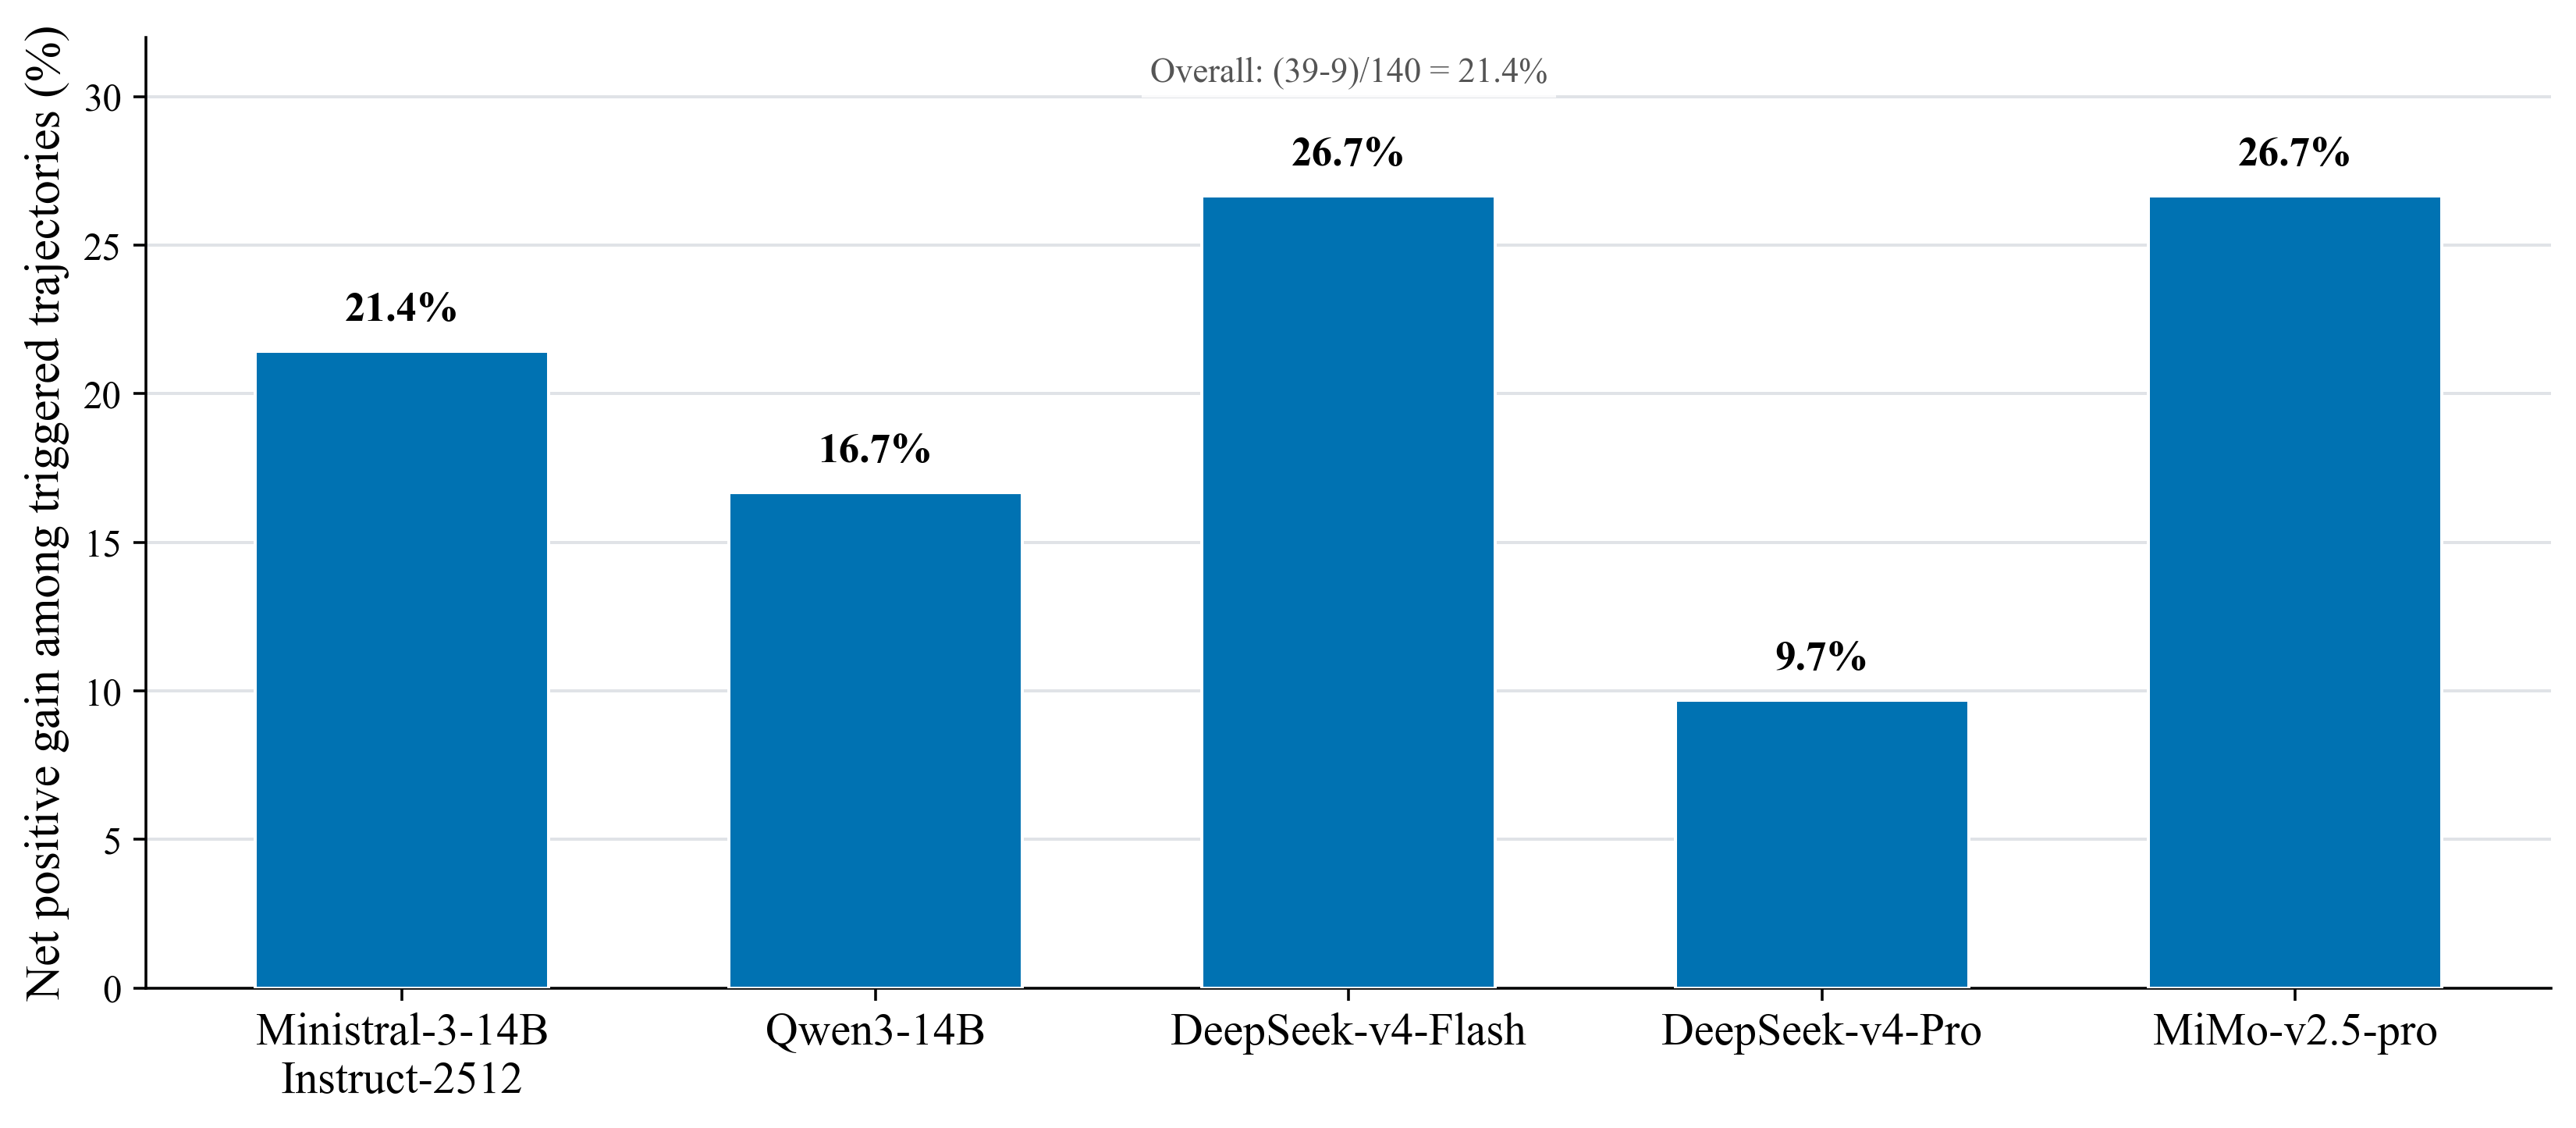
\includegraphics[width=\columnwidth]{figures/fig_statebench_triggered_failure_recovery.png}
\caption{Net outcome gain among triggered STATE-Bench trajectories. Each bar
reports $(W-L)/N_{\mathrm{triggered}}$ from paired Raw and PERSIST-ACE runs.
The overall margin is $(39-9)/140=21.4\%$.}
\label{fig:triggered-failure-recovery}
\end{figure}

\textbf{Triggered trajectories.}
Figure~\ref{fig:triggered-failure-recovery} shows a positive net outcome margin
for every model. Across 140 triggered trajectories, PERSIST-ACE produces 39
wins and 9 losses, yielding 30 net gains. The magnitude varies with the base
model, but the consistently positive direction indicates that the frozen
Registry transfers beyond a single model family and that beneficial
interventions outnumber harmful ones on the triggered subset.

\begin{figure}[!t]
\centering
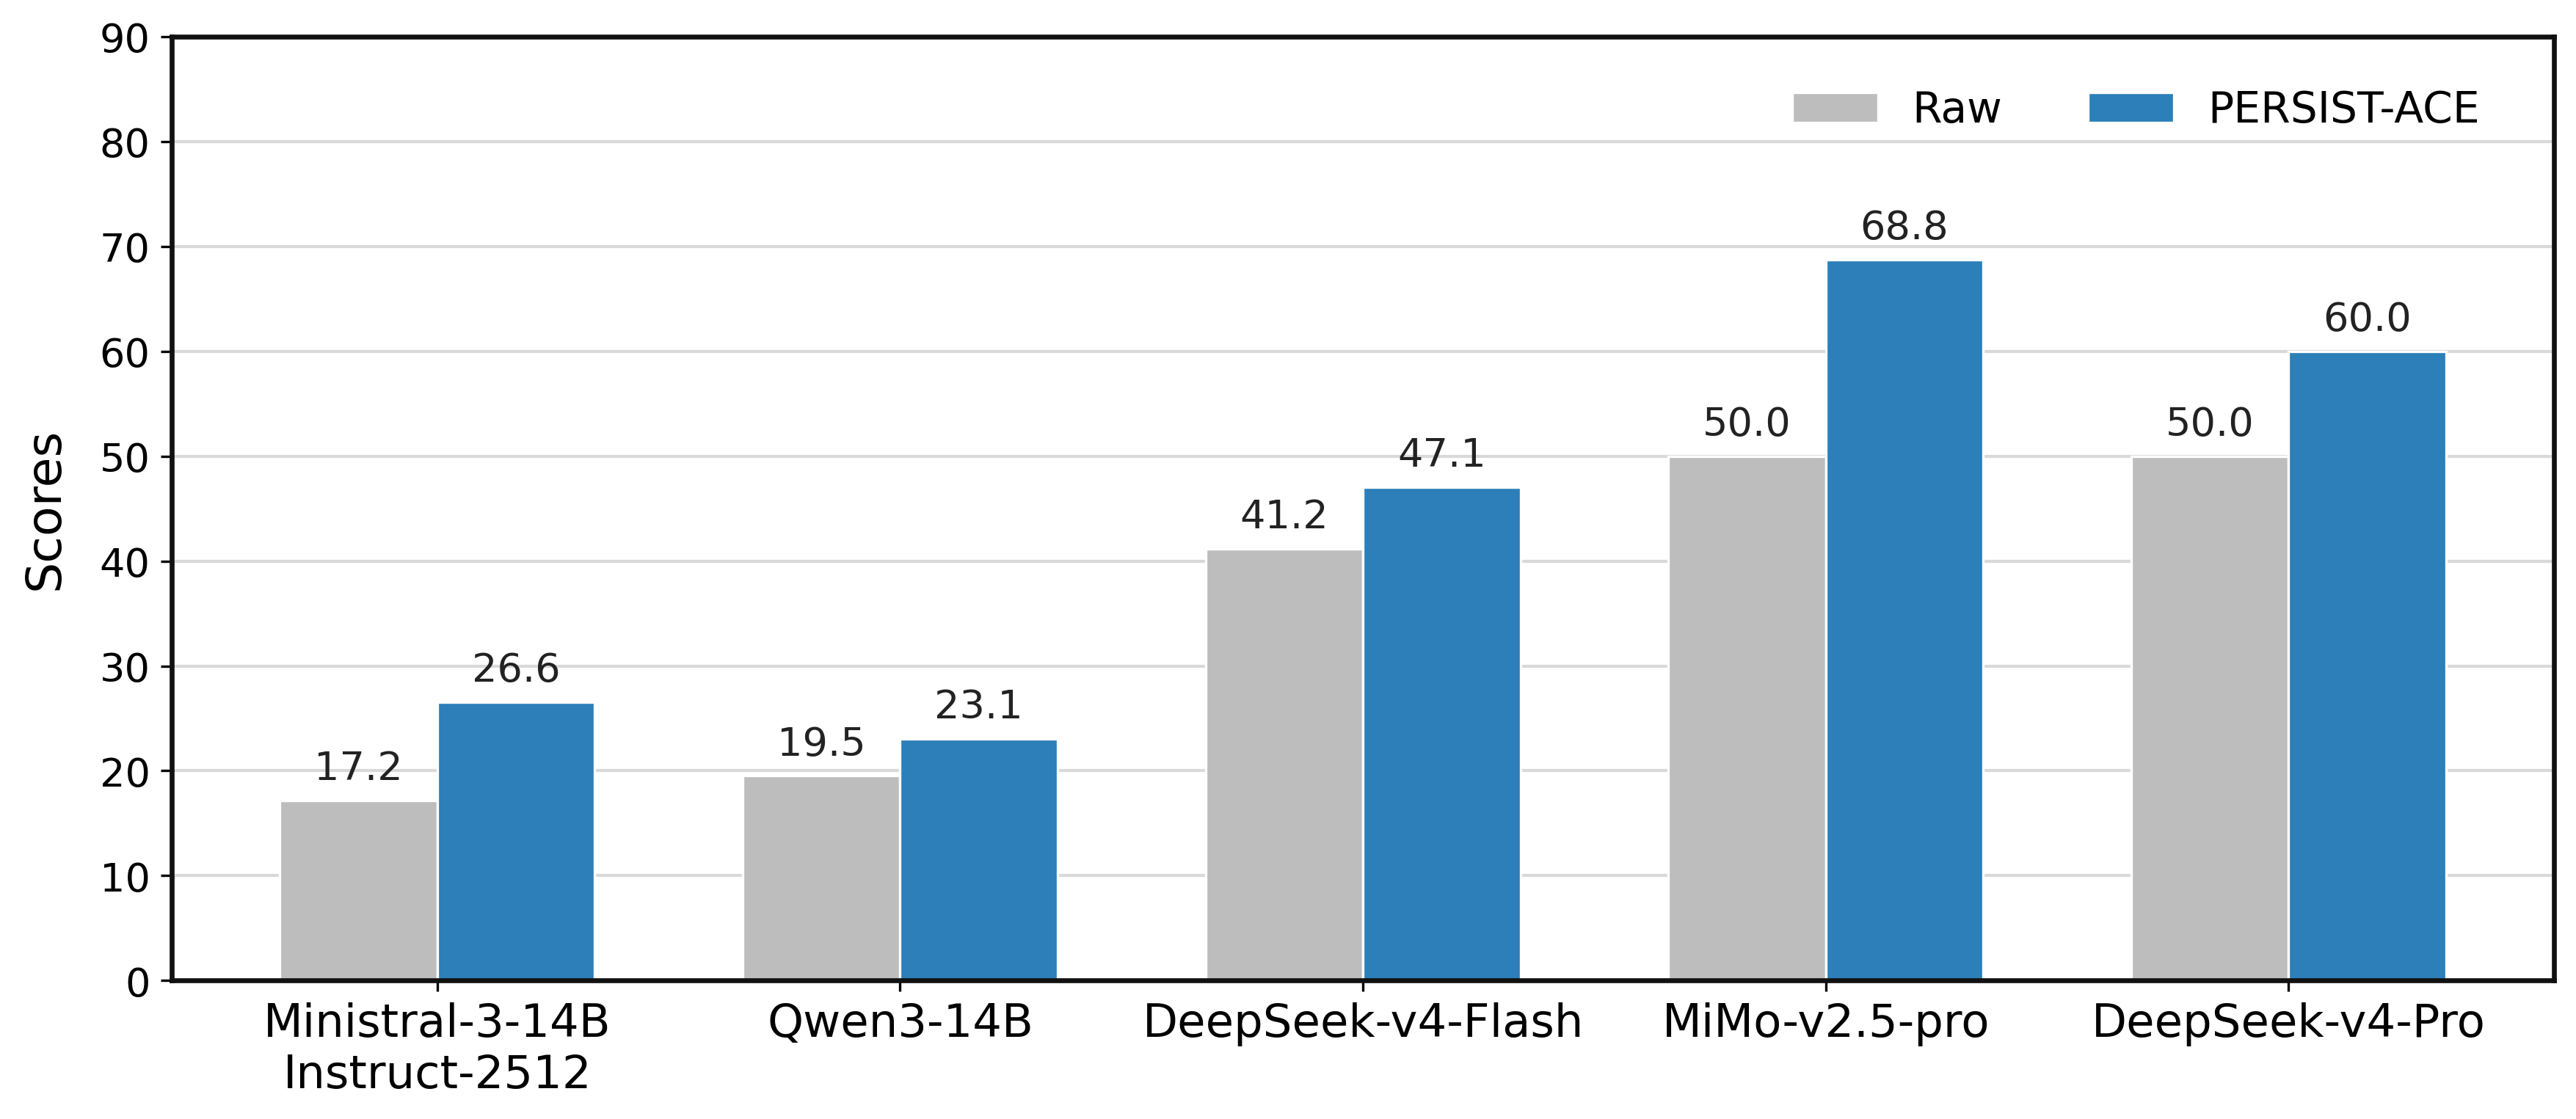
\includegraphics[width=\columnwidth]{figures/fig_statebench_fl_subset_scores.png}
\caption{STATE-Bench scores on task-runs whose Raw trajectory contains a
Functional Loop before intervention. PERSIST-ACE raises the score for all five
base models.}
\label{fig:functional-loop-subset-scores}
\end{figure}

\begin{figure}[!t]
\centering
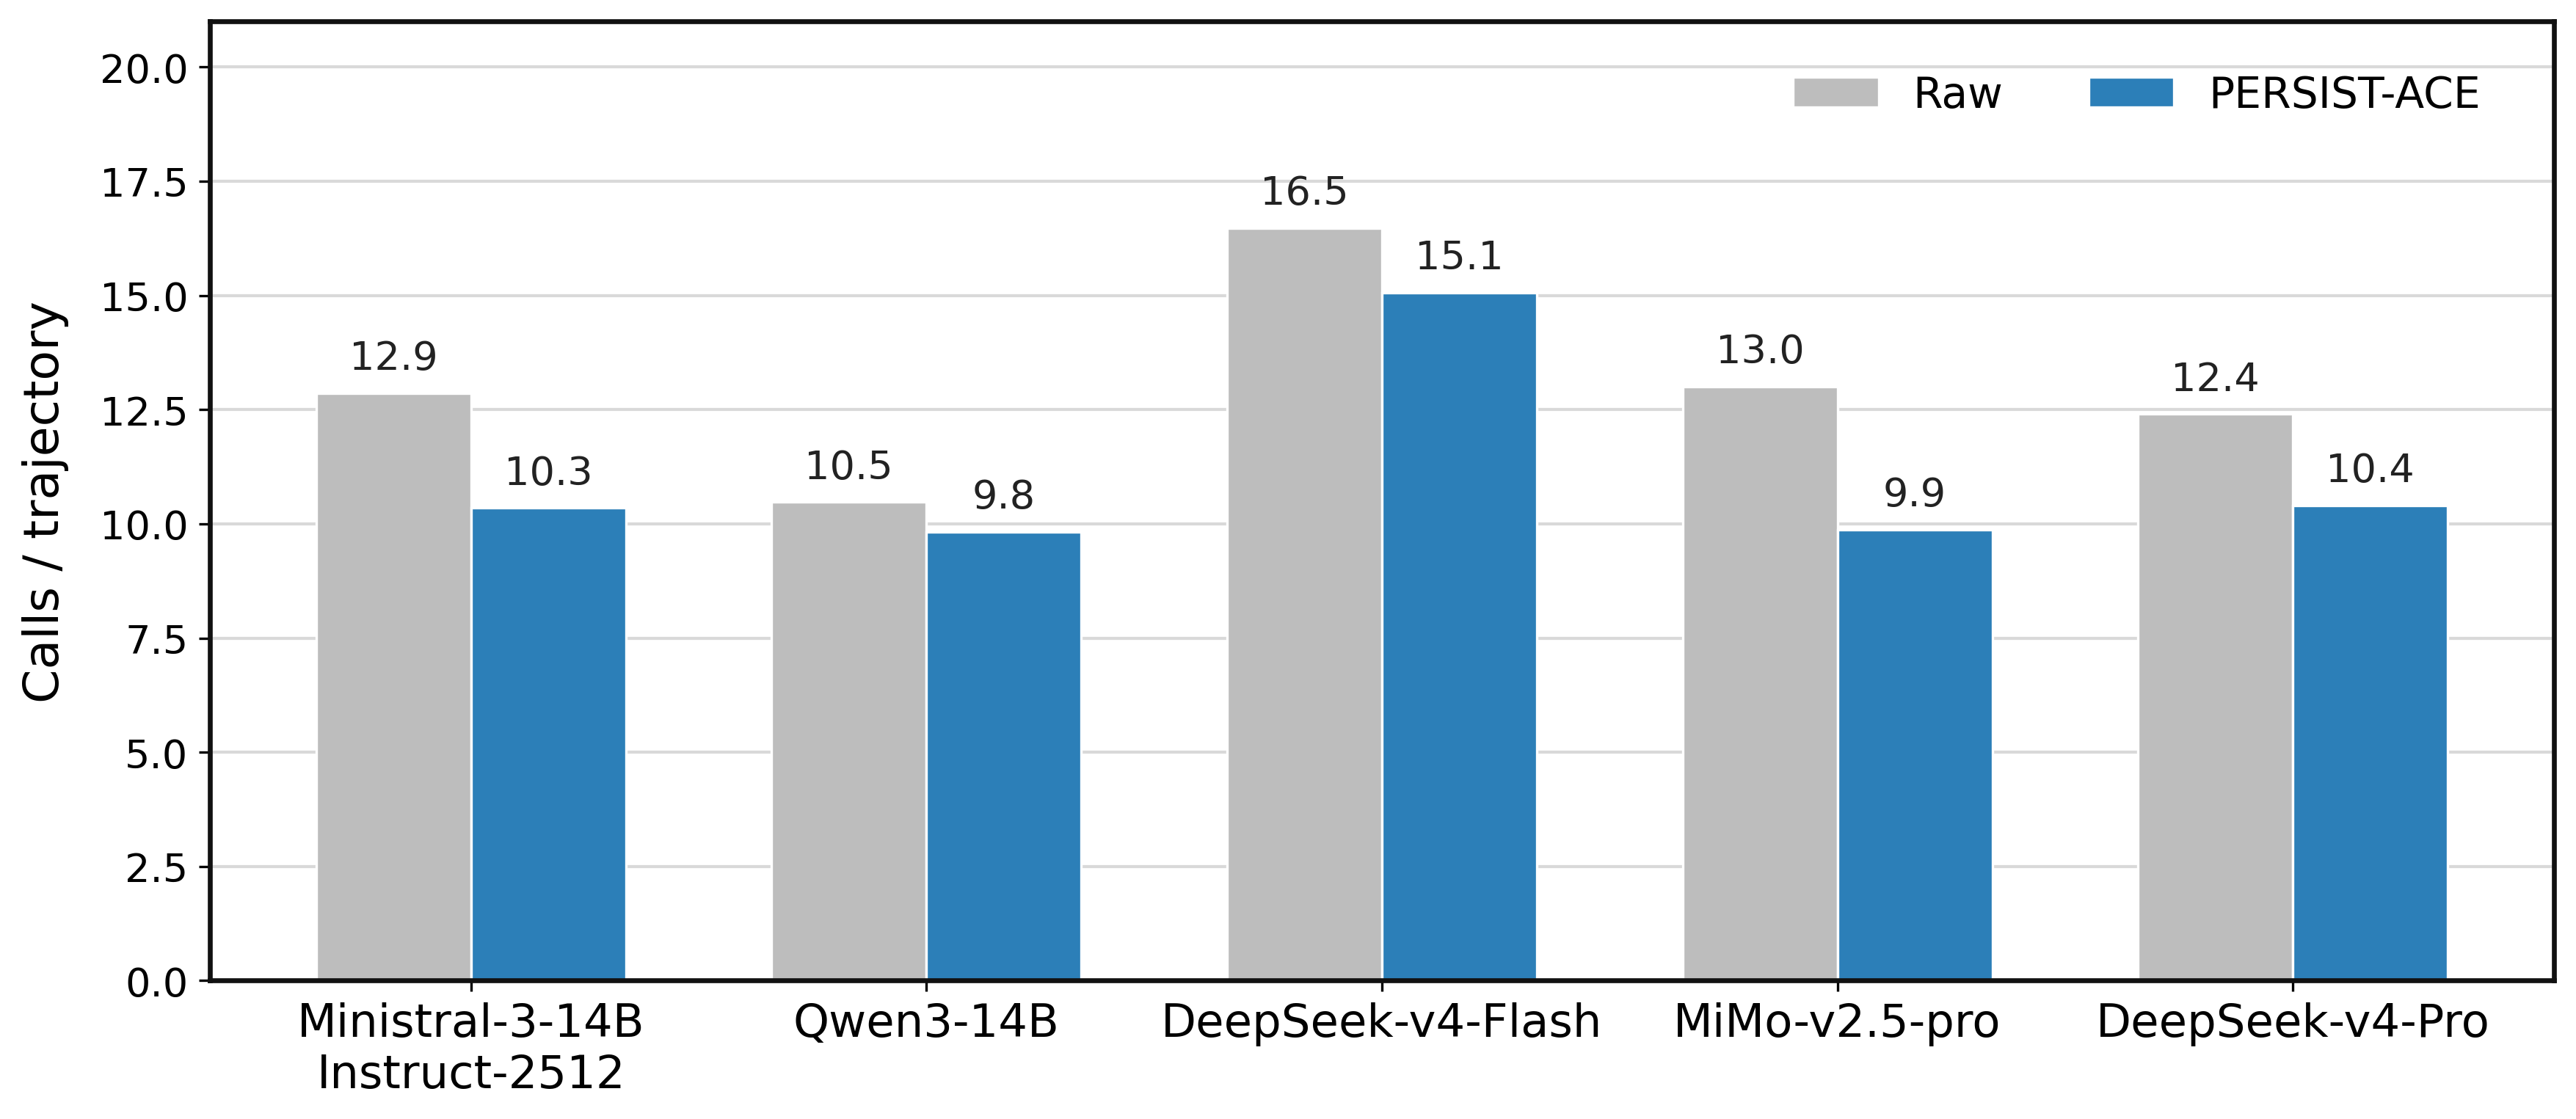
\includegraphics[width=\columnwidth]{figures/fig_statebench_fl_subset_calls.png}
\caption{Tool calls on the same Functional Loop-exposed task-runs used in
Figure~\ref{fig:functional-loop-subset-scores}. PERSIST-ACE reduces mean calls
for every base model.}
\label{fig:functional-loop-subset-calls}
\end{figure}

\textbf{Functional Loop-exposed trajectories.}
Figures~\ref{fig:functional-loop-subset-scores} and
\ref{fig:functional-loop-subset-calls} examine the subset that contained a
Functional Loop before intervention. Scores rise for all five models,
including lower- and higher-performing baselines, while tool calls fall in every
case. The largest score gains appear for MiMo-v2.5-Pro and DeepSeek-v4-Pro,
whereas even the smaller gains are accompanied by shorter trajectories. The
improvement is therefore not obtained by simply extending stalled runs. On the
subset identified by Functional Loops, PERSIST-ACE consistently reaches better
outcomes with less interaction, supporting the combination of Functional Loop
detection and grounded Card execution.

These subset results describe deployment behavior rather than an
action-level causal effect. The same-state experiment in
Table~\ref{tab:card-structure-ablation} provides the controlled evidence for
the recovery program itself.

\FloatBarrier

\section{Conclusion}

Functional Loops capture a failure mode that tool-name repetition misses:
after feedback is visible, tool-using LLMs may issue different calls that make no
progress and repeat the same unresolved functional effect. This matters because
the model continues spending interaction budget without changing the state
that blocks completion. The pattern depends on both the model and the
environment, and a Functional Loop can still precede a useful retry. On STATE-Bench,
however, Functional Loop-exposed trajectories are associated with lower scores and more
calls. A Functional Loop is therefore a useful recovery signal, but not a reason to
terminate every loop.

The experiments show a consistent task-level benefit. Every reported
Raw/PERSIST-ACE pair improves its primary outcome across STATE-Bench,
DeepPlanning Shopping, and $\tau$-Knowledge. The trend persists when different
models are evaluated on the same benchmark and when the same model is evaluated
on different benchmarks. Better outcomes do not require uniformly longer successful runs:
calls per successful trajectory usually decrease and otherwise remain close.
The ablations further locate the advantage in the recovery design. Online
Replanning with a generic prompt does not recover the baseline, the Validated Registry intervenes
more selectively and with lower observed loss than the Unvalidated All-Card
Registry, and complete Cards outperform operator-only and ungrounded variants
in held-out same-state comparisons. Independently removing the soft controller
gate increases coverage but not task performance.

Taken together, the results show why a Functional Loop is a practical unit for LLM tool-use
recovery. No progress recalls a candidate; repeated effect confirms the Functional Loop;
Card admission then decides whether it is recoverable. Across heterogeneous
models and tool environments, this separation improves task outcomes while
protecting productive retries and avoiding systematic growth in
successful-trajectory interaction cost.


\bibliography{references}

\end{document}
